\chapter{Mantle as a File System Metadata Load Balancer}
\label{mantle}

%%%%%%%%%%%%%%%%%%%%%%%%%%%%%%%%%%%%%%%%%%%%%%%%%%%%%%%%%%%%%%%%%%
\section{Introduction}								    %%%%%%%%%%
\label{introduction}								    %%%%%%%%%%
%%%%%%%%%%%%%%%%%%%%%%%%%%%%%%%%%%%%%%%%%%%%%%%%%%%%%%%%%%%%%%%%%%
% What is the metadata management problem?
Serving metadata and maintaining a POSIX namespace is challenging for large-scale distributed file systems because accessing metadata imposes small and frequent requests on the underlying storage system~\cite{roselli:atec2000-FS-workloads}. As a result of this skewed workload, serving metadata requests does not scale for sufficiently large systems in the same way that read and write throughput do~\cite{abad:ucc2012-mimesis, alam:pdsw2011-metadata-scaling, weil:osdi2006-ceph}. Many distributed file systems decouple metadata from data access so that data and metadata I/O can scale independently~\cite{alam:pdsw2011-metadata-scaling, ghemawat:sosp2003-gfs, hildebrand:msst2005-pnfs,weil:osdi2006-ceph,welch:fast2008-panasas,xing:sc2009-skyfs}. These ``metadata services" manage the namespace hierarchy and metadata requests ({\it e.g.}, file and directory creates, file and directory renaming, directory listings). File properties that a metadata service manages can include permissions, size, modification times, link count, and data location. 

%konstantinos:pdsw2014-lustre-metadata

\begin{figure}[tb]
	\centering	
	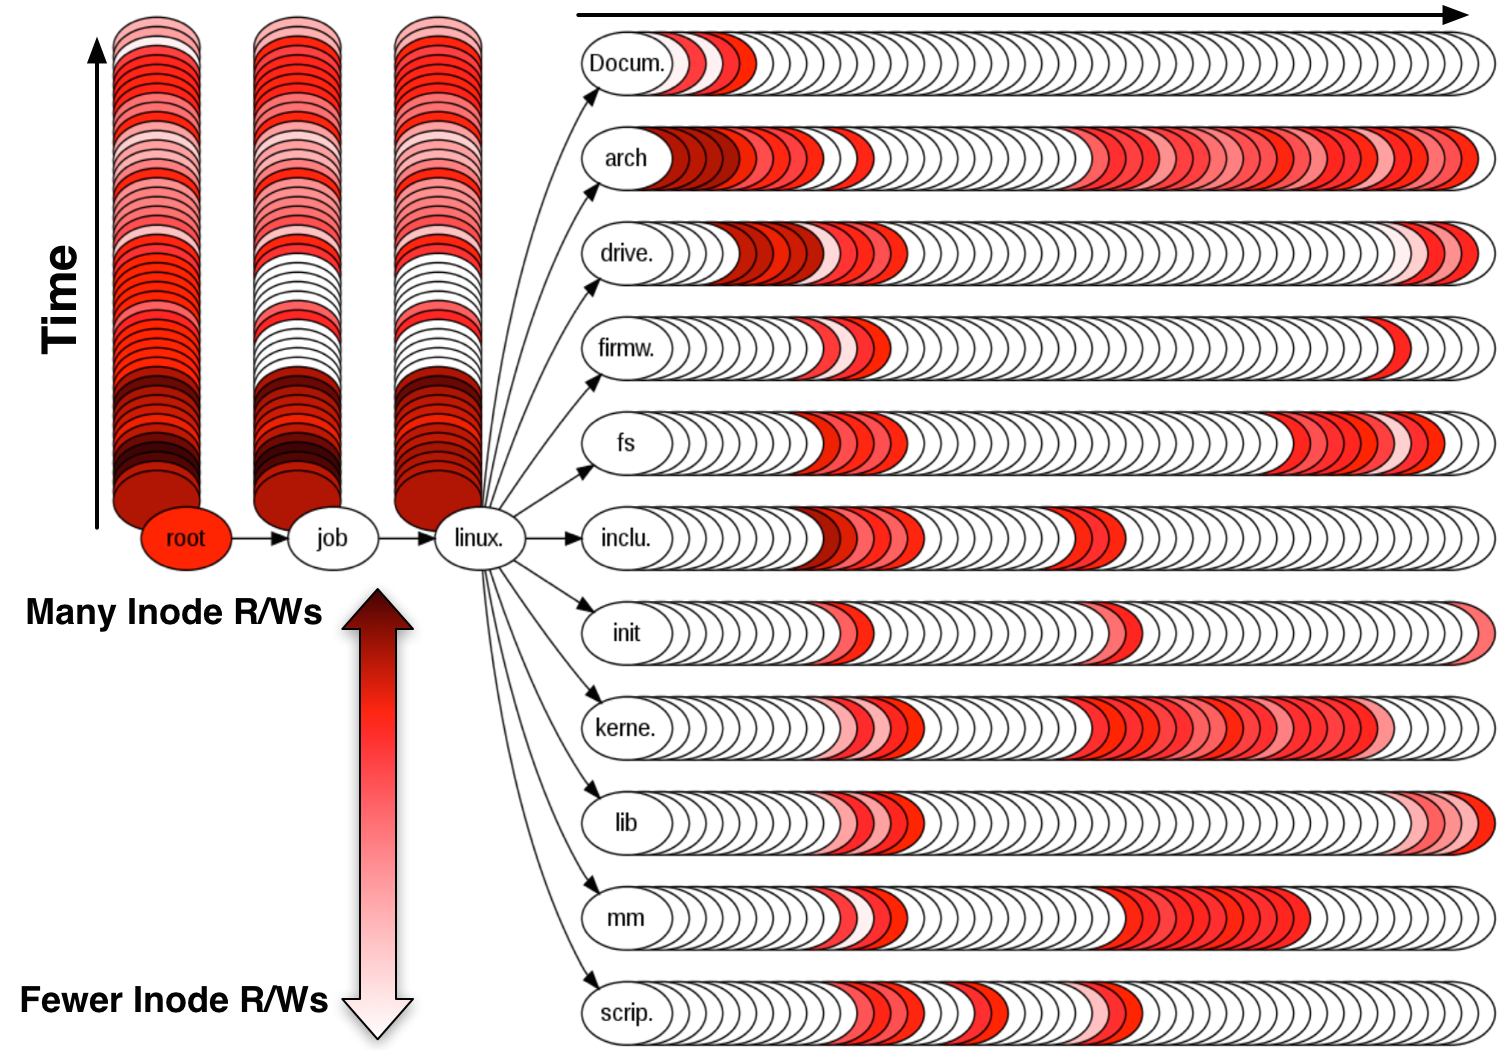
\includegraphics[width=0.5\textwidth]{./chapters/mantle/workload-tar.png}
	\caption{Metadata hotspots, represented by different shades of red, have spatial and temporal locality when compiling the Linux source code. The hotspots are calculated using the number of inode reads/writes and smoothed with an exponential decay. \label{figure:workload-tar}}
\end{figure}

% Why you should care: metadata management as a resurgence
Unfortunately, decoupling metadata and data is insufficient for scaling and many setups require customized application solutions for dealing with metadata intensive workloads. For example, Google has acknowledged a strain on their own metadata services because their workloads involve many small files ({\it e.g.}, log processing) and simultaneous clients ({\it e.g.}, MapReduce jobs)~\cite{mckusick:acm2010-gfs-evolution}. Metadata inefficiencies have also plagued Facebook; they migrated away from file systems for photos~\cite{beaver:osdi2010-haystack} and aggressively concatenate and compress small files so that their Hive queries do not overload the HDFS namenode~\cite{thusoo:sigmod2010-facebook-infrastructure}. The elegance and simplicity of the solutions stem from a thorough understanding of the workloads ({\it e.g.}, temperature zones at Facebook~\cite{muralidhar:osdi2014-f4}) and are not applicable for general purpose storage systems. 

% Multi-MDS problem: synchronizing access and coalescing knowledge 
The most common technique for improving the performance of these metadata services is to balance the load across dedicated metadata server (MDS) nodes~\cite{patil:fast2011-giga+,weil:osdi2006-ceph,weil:sc2004-dyn-metadata,sinnamohideen:atc2010-ursa,xing:sc2009-skyfs}. Distributed MDS services focus on parallelizing work and synchronizing access to the metadata. A popular approach is to encourage independent growth and reduce communication, using techniques like lazy client and MDS synchronization~\cite{patil:fast2011-giga+, ren:sc2014-indexfs, zheng:pdsw2014-batchfs, hildebrand:msst2005-pnfs, zhu:pds2008-hba}, inode path/permission caching~\cite{brandt:mss2003-lh, li:msst2006-dynamic, xing:sc2009-skyfs}, locality-aware/inter-object transactions~\cite{sinnamohideen:atc2010-ursa,zhu:pds2008-hba,ren:atc2013-tablefs, ren:sc2014-indexfs} and efficient lookup tables~\cite{brandt:mss2003-lh, zhu:pds2008-hba}. Despite having mechanisms for migrating metadata, like locking~\cite{sinnamohideen:atc2010-ursa,schmuck:fast2002-gpfs}, zero copying and two-phase commits~\cite{sinnamohideen:atc2010-ursa}, and directory partitioning~\cite{xing:sc2009-skyfs, patil:fast2011-giga+, ren:sc2014-indexfs, weil:osdi2006-ceph}, these systems fail to exploit locality.

% Locality is a big part of workloads
File system workloads have locality because the namespace has semantic meaning; data stored in directories is related and is usually accessed together. Figure~\ref{figure:workload-tar} shows the metadata locality when compiling the Linux source code. The ``heat" of each directory is calculated with per-directory metadata counters, which are tempered with an exponential decay. The hotspots can be correlated with phases of the job: untarring the code has high, sequential metadata load across directories and compiling the code has hotspots in the \texttt{arch}, \texttt{kernel}, \texttt{fs}, and \texttt{mm} directories. Exploiting this locality has positive implications for performance because it reduces the number of requests, lowers the communication across MDS nodes, and eases memory pressure. The Ceph~\cite{weil:osdi2006-ceph} (see also www.ceph.com) file system (CephFS) tries to leverage this spatial, temporal, and request-type locality in metadata intensive workloads using dynamic subtree partitioning, but struggles to find the best degree of locality and balance.

% ... and what we do
We envision a general purpose metadata balancer that responds to many types of parallel applications. To get to that balancer, we need to understand the trade-offs of resource migration and the processing capacity of the MDS nodes. We present Mantle\footnote{The mantle is the structure behind an octopus's head that protects its organs.}, a system built on CephFS that exposes these factors by separating migration policies from the mechanisms. Mantle accepts injectable metadata migration code and helps us make the following contributions:

\begin{itemize}
	\item a comparison of balancing for locality and balancing for distribution
    \item a general framework for succinctly expressing different load balancing techniques 
    \item an MDS service that supports simple balancing scripts using this framework
\end{itemize}

Using Mantle, we can dynamically select different techniques for distributing metadata. We explore the infrastructures for a better understanding of how to balance diverse metadata workloads and ask the question ``is it better to spread load aggressively or to first understand the capacity of MDS nodes before splitting load at the right time under the right conditions?''. We show how the second option can lead to better performance but at the cost of increased complexity. We find that the cost of migration can sometimes outweigh the benefits of parallelism (up to 40\% performance degradation) and that searching for balance too aggressively increases the standard deviation in runtime.

%%%%%%%%%%%%%%%%%%%%%%%%%%%%%%%%%%%%%%%%%%%%%%%%%%%%%%%%%%%%%%%%%%
\section{Background: Dynamic Subtree Partitioning}	%%%%%%%%%%
\label{background_dynamic_subtree_partitioning}			%%%%%%%%%%
%%%%%%%%%%%%%%%%%%%%%%%%%%%%%%%%%%%%%%%%%%%%%%%%%%%%%%%%%%%%%%%%%%
\begin{figure}[tb]
	\centering	
	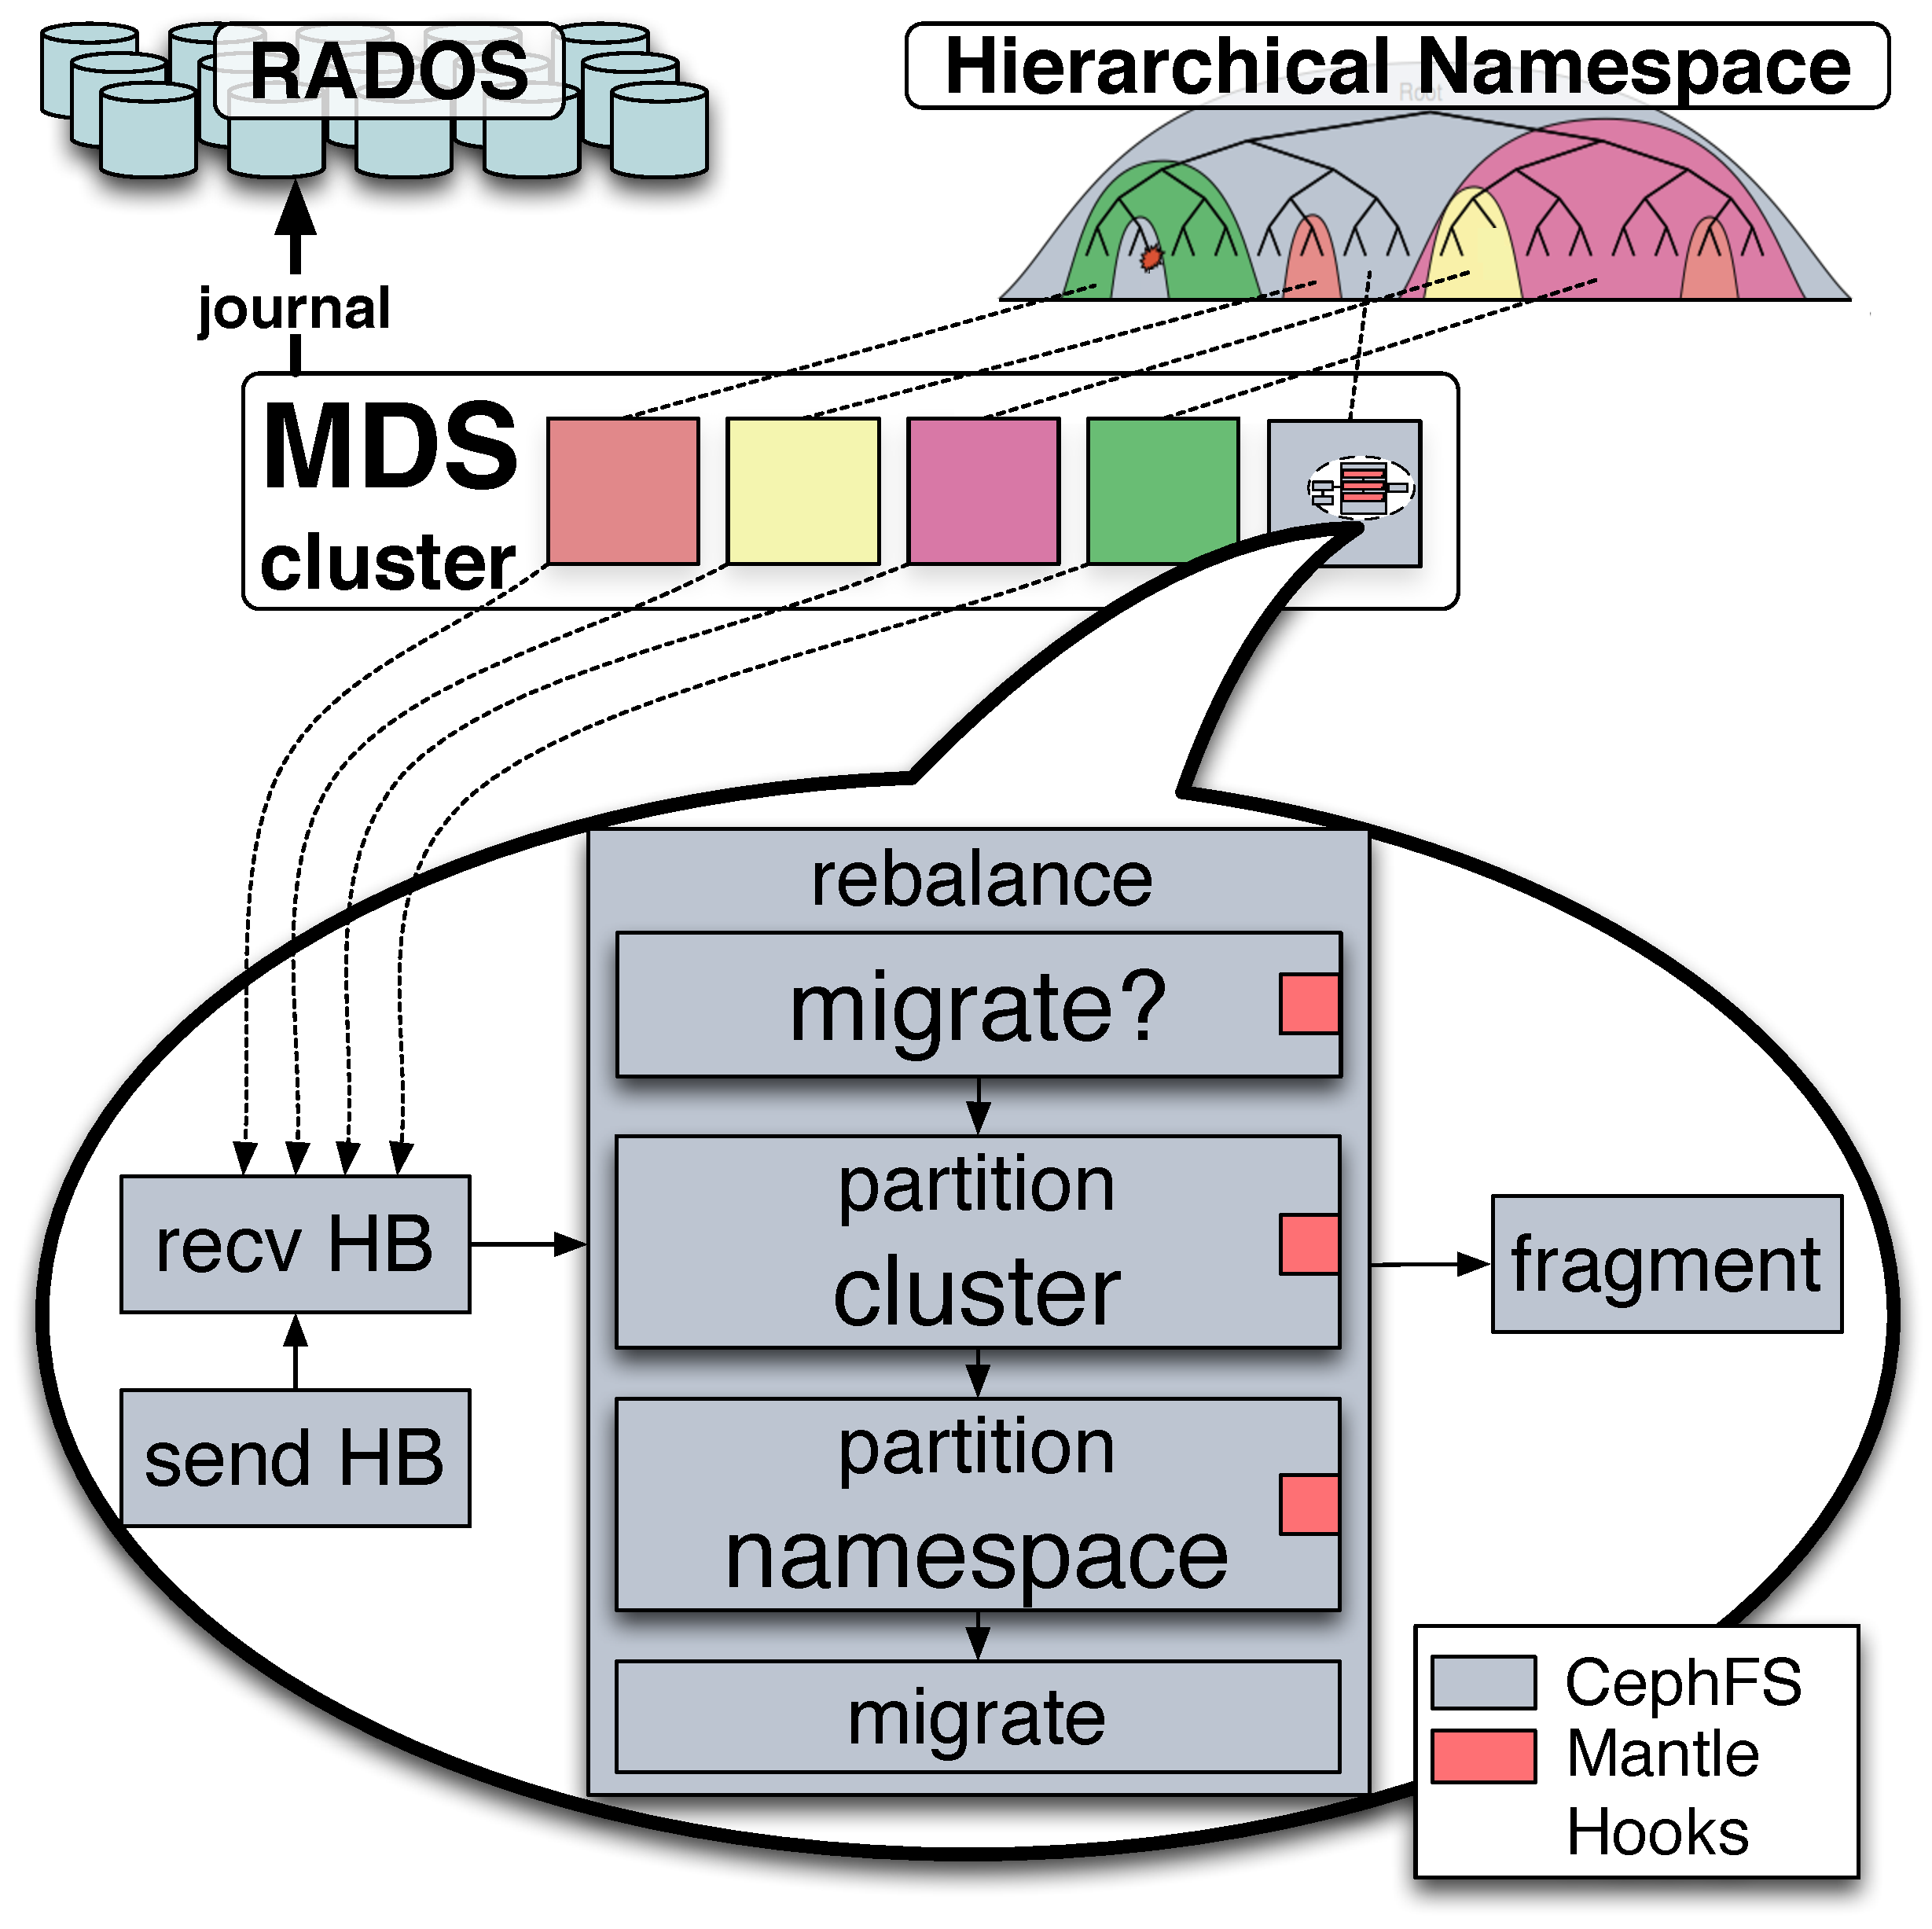
\includegraphics[width=0.4\textwidth]{./chapters/mantle/balancer-diagram.pdf}
 	\caption{The MDS cluster journals to RADOS and exposes a namespace to clients. Each MDS makes decisions by exchanging heartbeats and partitioning the cluster/namespace. Mantle adds code hooks for custom balancing logic.\label{figure:balancer-diagram}}    
\end{figure}   

% Ceph background
We use Ceph~\cite{weil:osdi2006-ceph} to explore the metadata management problem. Ceph is a distributed storage platform that stripes and replicates data across a reliable object store called RADOS. Clients talk directly to object storage daemons (OSDs) on individual disks by calculating the data placement (``where" should I store my data) and location (``where" did I store my data) using a hash-based algorithm (CRUSH). CephFS is the POSIX-compliant file system that uses RADOS. It decouples metadata and data access, so data IO is done directly with RADOS while all metadata operations go to a separate metadata cluster. The MDS cluster is connected to RADOS so it can periodically flush its state. The hierarchical namespace is kept in the collective memory of the MDS cluster and acts as a large distributed cache. Directories are stored in RADOS, so if the namespace is larger than memory, parts of it can be swapped out. 

% Outline of the figure.
The MDS nodes use dynamic subtree partitioning~\cite{weil:sc2004-dyn-metadata} to carve up the namespace and to distribute it across the MDS cluster, as shown in Figure~\ref{figure:balancer-diagram}. MDS nodes maintain the subtree boundaries and ``forward" requests to the authority MDS if a client's request falls outside of its jurisdiction or if the request tries to write to replicated metadata.  Each MDS has its own metadata balancer that makes independent decisions, using the flow in Figure~\ref{figure:balancer-diagram}.  Every 10 seconds, each MDS packages up its metrics and sends a heartbeat (``send HB") to every MDS in the cluster. Then the MDS receives the heartbeat (``recv HB'') and incoming inodes from the other MDS nodes. Finally, the MDS decides whether to balance load (``rebalance'') and/or fragment its own directories (``fragment"). If the balancer decides to rebalance load, it partitions the namespace and cluster and sends inodes (``migrate'') to the other MDS nodes. These last 3 phases are discussed below.

% Migrate
\textbf{Migrate}: inode migrations are performed as a two-phase commit, where the importer (MDS node that has the capacity for more load) journals metadata, the exporter (MDS node that wants to shed load) logs the event, and the importer journals the event. Inodes are embedded in directories so that related inodes are fetched on a \texttt{readdir} and can be migrated with the directory itself.

% Partitioning the namespace
\textbf{Partitioning the Namespace}: each MDS node's balancer carves up the namespace into {\it subtrees} and {\it directory fragments} (added since~\cite{weil:sc2004-dyn-metadata,weil:osdi2006-ceph}). Subtrees are collections of nested directories and files, while directory fragments ({\it i.e.} dirfrags) are partitions of a single directory; when the directory grows to a certain size, the balancer fragments it into these smaller dirfrags. This directory partitioning mechanism is equivalent to the GIGA+~\cite{patil:fast2011-giga+} mechanism, although the policies for moving the dirfrags can differ.  These subtrees and dirfrags allow the balancer to  partition the namespace into fine- or coarse-grained units.

% How does the balancer partition the namespace: metadata load
Each balancer constructs a local view of the load by identifying popular subtrees or dirfrags using metadata counters. These counters are stored in the directories and are updated by the MDS whenever a namespace operation hits that directory or any of its children. Each balancer uses these counters to calculate a {\it metadata load} for the subtrees and dirfrags it is in charge of (the exact policy is explained in Section~\S\ref{the-cephfs-policies}). The balancer compares metadata loads for different parts of its namespace to decide which inodes to migrate. Once the balancer figures out which inodes it wants to migrate, it must decide where to move them.

% What is partitioning cluster
\textbf{Partitioning the Cluster}: each balancer communicates its metadata load and resource metrics to every other MDS in the cluster. Metadata load metrics include the metadata load on the root subtree, the metadata load on all the other subtrees, the request rate/latency, and the queue lengths. Resource metrics include measurements of the CPU utilization and memory usage. The balancer calculates an {\it MDS load} for all MDS nodes using a weighted sum of these metrics (again, the policy is explained in Section~\S\ref{the-cephfs-policies}), in order to quantify how much work each MDS is doing. With this global view, the balancer can partition the cluster into exporters and importers. These loads also help the balancer figure out which MDS nodes to ``target'' for exporting and {\it how much} of its local load to send. The key to this load exchange is the load calculation itself, as an inaccurate view of another MDS or the cluster state can lead to poor decisions.

\textbf{CephFS's Client-Server Metadata Protocols}: the mechanisms for migrating metadata, ensuring consistency, enforcing synchronization, and mediating access are discussed at great length in~\cite{weil:phdthesis07} and the Ceph source code. MDS nodes and clients cache a configurable number of inodes so that requests like \texttt{getattr} and \texttt{lookup} can resolve locally.  For shared resources, MDS nodes have coherency protocols implemented using scatter-gather processes. These are conducted in sessions and involve halting updates on a directory, sending stats around the cluster, and then waiting for the authoritative MDS to send back new data. As the client receives responses from MDS nodes, it builds up its own mapping of subtrees to MDS nodes. 

%%%%%%%%%%
\subsection{Advantages of Locality}
\label{advantages_of_locality}
%%%%%%%%%%
\begin{figure*}[tbh]
	\begin{subfigure}[H]{0.45\textwidth}
		\centering	
	\caption{The number of requests for the compile job.  \label{figure:workload-tar-requests-total}}
		
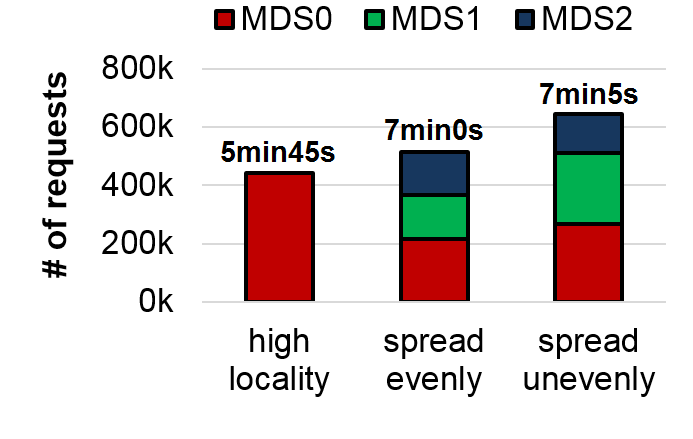
\includegraphics[width=1\textwidth]{./chapters/mantle/workload-tar-requests2.png}
	\end{subfigure}
	~
	\begin{subfigure}[H]{0.47\textwidth}
		\centering
		\caption{Path traversals ending in hits (local metadata) and forwards. \label{figure:workload-tar-traverses}}	
	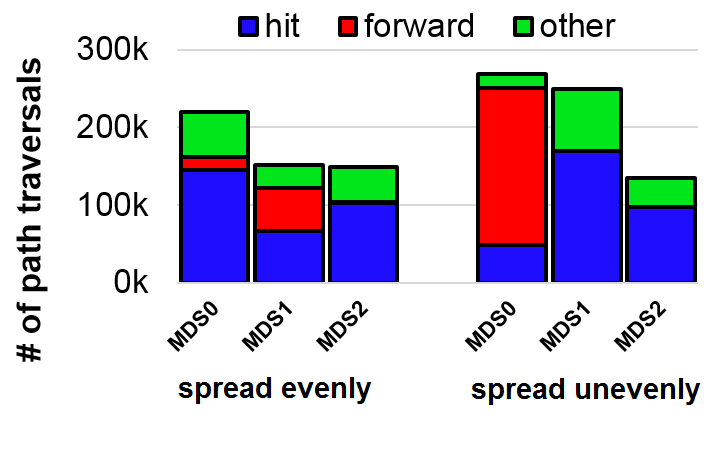
\includegraphics[width=1\textwidth]{./chapters/mantle/workload-tar-traverses2.png}
	\end{subfigure}	
	\caption{Spreading metadata to multiple MDS nodes hurts performance (``spread evenly/unevenly" setups in Figure 3a) when compared to keeping all metadata on one MDS (``high locality'' setup in Figure 3a). The times given are the total times of the job (compile, read, write, etc.). Performance is worse when metadata is spread unevenly because it ``forwards" more requests (Figure 3b).\label{figure:workload-tar-requests}}
\end{figure*}

% Distribution hurts performance
Distributing metadata for balance tries to spread metadata evenly across the metadata cluster. The advantage of this approach is that clients can contact different servers for their metadata in parallel. Many metadata balancers distribute metadata for complete balance by hashing a unique identifier, like the inode or filename; unfortunately, with such fine grain distribution, locality is completely lost. Distributing for locality keeps related metadata on one MDS and can improve performance. The reasons are discussed in ~\cite{weil:phdthesis07, weil:sc2004-dyn-metadata}, but briefly, improving locality can: 
\begin{itemize}
	\item reduce the number of forwards between MDS nodes ({\it i.e.} requests for metadata outside the MDS node's jurisdiction)
	\item lower communication for maintaining coherency ({\it i.e.} requests involving prefix path traversals and permission checking)
	\item reduce the amount of memory needed to cache path prefixes. If metadata is spread, the MDS cluster replicates parent inode metadata so that path traversals can be resolved locally
\end{itemize}

% Example
Figure~\ref{figure:workload-tar-requests} alters the degree of locality by changing how metadata is distributed for a client compiling code on CephFS; with less locality, the performance gets worse and the number of requests increases. The number of requests ({\it y} axis) increases when metadata is distributed: the ``high locality" bar is when all metadata is kept on one MDS, the ``spread evenly" bar is when hot metadata is correctly distributed, and the ``spread unevenly" bar is when hot metadata is incorrectly distributed\footnote{To get high locality, all metadata is kept on one MDS. To get different degrees of spread, we change the setup: ``spread unevenly'' is untarring and compiling with 3 MDS nodes and ``spread evenly'' is untarring with 1 MDS and compiling with 3 MDS nodes. In the former, metadata is distributed when untarring (many creates) and the workload loses locality.}. For this example, the speedup for keeping all metadata on a single MDS is between 18\% and 19\%. Although this is a small experiment, where the client clearly does not overload one MDS, it demonstrates how unnecessary distribution can hurt performance.

% Reason for improvement in performance
The number of requests increases when distributing metadata because the MDS nodes need to forward requests for remote metadata in order to perform common file system operations. The worse the distribution and the higher the fragmentation, the higher the number of forwards. Figure~\ref{figure:workload-tar-traverses} shows that a high number of path traversals ({\it y} axis) end in "forwards" to other MDS nodes when metadata is spread unevenly. When metadata is spread evenly, much more of the path traversals can be resolved by the current MDS ({\it i.e.} they are cache "hits"). Aggressively caching all inodes and prefixes can reduce the requests between clients and MDS nodes, but CephFS (as well as many other file systems) do not have that design, for a variety of reasons.

%%%%%%%%%%%%%%%%%%%%%%%%%%%%%%%%%%%%%%%%%%%%%%%%%%%%%%%%%%%%%%%%%%
\subsection{Multi-MDS Challenges}					    %%%%%%%%%%
\label{multi-mds_challenges}						    %%%%%%%%%%
%%%%%%%%%%%%%%%%%%%%%%%%%%%%%%%%%%%%%%%%%%%%%%%%%%%%%%%%%%%%%%%%%%
% ACTION ITEM: survey paper of load balancing
Dynamic subtree partitioning achieves varying degrees of locality and distribution by changing the way it carves up the namespace and partitions the cluster. To alleviate load quickly, dynamic subtree partitioning can move different sized resources (inodes) to computation engines with variable capacities (MDS nodes), but this flexibility has a cost. In the sections below, we describe CephFS's current architecture and demonstrate how its complexity limits performance. While this section may seem like an argument against dynamic subtree partitioning, our main conclusion is that the approach has potential and warrants further exploration. 

%%%%%%%%%%%%%%%%%%%%
\subsubsection{Complexity Arising from Flexibility}
\label{complexity-arising-from-flexibility}
%%%%%%%%%%%%%%%%%%%%

% The problem: load balancing is hard
The complexity of deciding where to migrate resources increases significantly if these resources have different sizes and characteristics. To properly balance load, the balancer must model how components interact. First, the model needs to be able to predict how different decisions will positively impact performance. The model should consider what can be moved and how migration units can be divided or combined. It should also  consider how splitting different or related objects affects performance and behavior. Second, the model must quantify the state of the system using available metrics. Third, the model must tie the metrics to the global performance and behavior of the system. It must consider how over-utilized resources negatively affect performance and how system events can indicate that the system is performing optimally. With such a model, the balancer can decide which metrics to optimize for.

% Basic overview of cluster and workloads
Figure~\ref{figure:creates-thruput} shows how a 10 node, 3 MDS CephFS system struggles to build an accurate model that addresses the challenges inherent to the metadata management problem. That figure shows the total cluster throughput ({\it y} axis) over time ({\it x} axis) for 4 runs of the same job: creating 100,000 files in separate directories. The top graph, where the load is split evenly, is what the balancer tries to do. The results and performance profiles of the other 3 runs demonstrate that the balancing behavior is not reproducible, as the finish times vary between 5 and 10 minutes and the load is migrated to different servers at different times in different orders. Below, we discuss the design decisions that CephFS made and we demonstrate how policies with good intentions can lead to poor performance and unpredictability.

% /user/msevilla/results/multimds/3mds-3client-sepdir/graphs/images/create-throughput_run5.pdf
\begin{figure}[tb]
	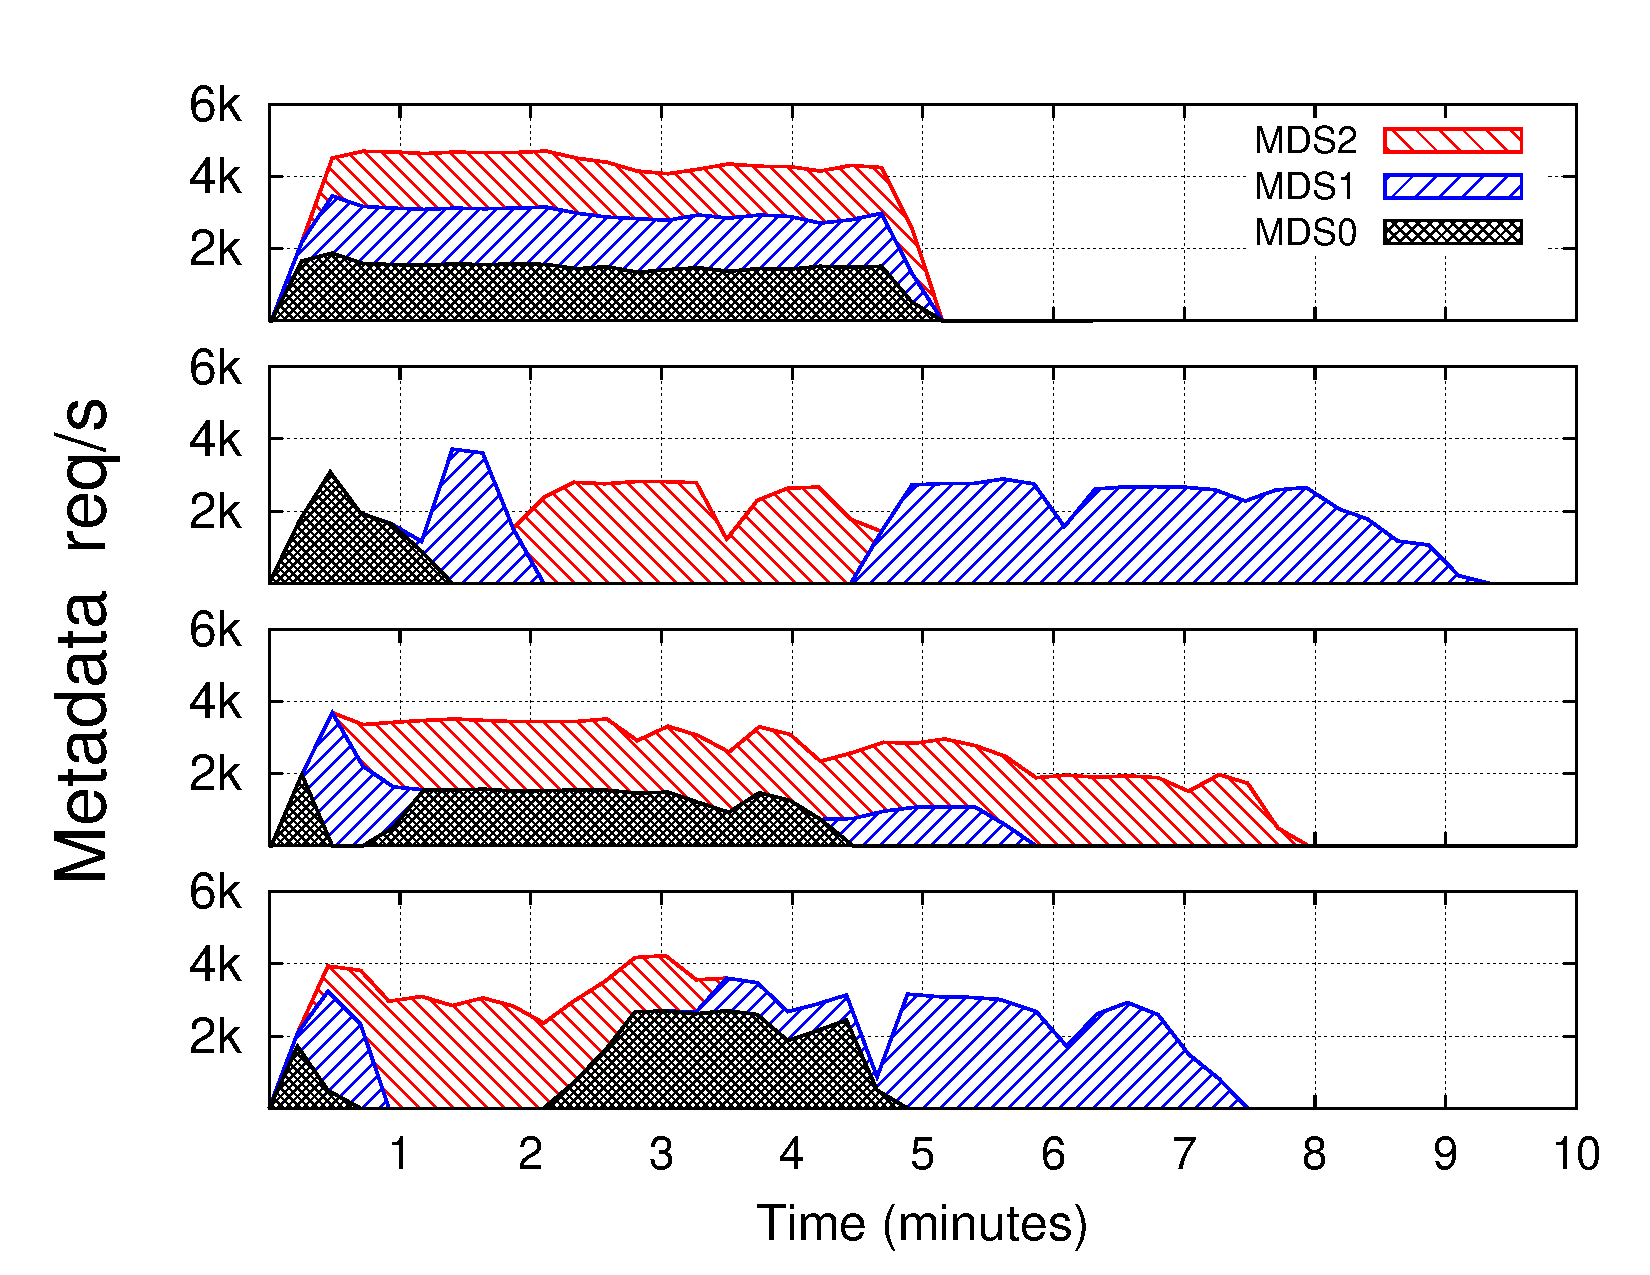
\includegraphics[width=0.45\textwidth]{./chapters/mantle/creates-thruput-runs2.pdf}
	\caption{The same create-intensive workload has different throughput ({\it y} axis; curves are stacked) because of how CephFS maintains state and sets policies.\label{figure:creates-thruput}}
\end{figure}
%%%%%%%%%%%%%%%%%%%%
\subsubsection{Maintaining Global \& Local State}
\label{the-challenge-in-maintaining_global_local_state}
%%%%%%%%%%%%%%%%%%%%

To make fast decisions, CephFS measures, collects, and communicates small amounts of state. Each MDS runs its balancing logic concurrently - this allows it to construct its own view of the cluster. The design decisions of the current balancer emphasizes speed over accuracy: 
\begin{enumerate}
	\item \textbf{Instantaneous measurements}: this makes the balancer sensitive to common system perturbations. The balancer can be configured to use CPU utilization as a metric for making decisions but this metric depends on the instant the measurement is taken and can be influenced by the measurement tool. The balancer dulls this effect by comparing the current measurement against the previous measurement, but in our experiences decisions are still made too aggressively. 
	\item \textbf{Decentralized MDS state}: this makes the balancers reliant on state that is slightly stale. CephFS communicates the load of each MDS around the cluster using heartbeats, which take time to pack, travel across the network, and unpack. As an example, consider the instant MDS0 makes the decision to migrate some of its load; at this time, that MDS considers the aggregate load for the whole cluster by looking at all incoming heartbeats, but by the time MDS0 extracts the loads from all these heartbeats, the other MDS nodes have already moved on to another task. As a result of these inaccurate and stale views of the system, the accuracy of the decisions varies and reproducibility is difficult. 
\end{enumerate}

Even if maintaining state was instant and consistent, making the correct migration decisions would still be difficult because the workload itself constantly changes.

%%%%%%%%%%%%%%%%%%%%
\subsubsection{Setting Policies for Migration Decisions}
\label{setting-policies-for-migration-decisions}
%%%%%%%%%%%%%%%%%%%%
\begin{table}[tb]
	\centering
	\begin{tabular}{ >{}p{1.5cm} | >{}p{6.8cm}}
		\centering\textbf{Policy} & \centering\textbf{Hard-coded implementation}
		\tabularnewline\hline		
		metaload	 	& \small{\texttt{= inode reads + 2*(inode writes)}}\tabularnewline
					 	& \small{\texttt{~~+ read dirs + 2*fetches + 4*stores}}\tabularnewline        
		MDSload      	& \small{\texttt{= 0.8*(metaload on auth)}}\tabularnewline
        				& \small{\texttt{~~+ 0.2*(metaload on all)}}\tabularnewline
        				& \small{\texttt{~~+ request rate + 10*(queue length)}}\tabularnewline
		when			& \small{\texttt{if my load \(>\) (total load)/\#MDSs}}\tabularnewline
        
		where			& \small{\texttt{for each MDS}}\tabularnewline	
          			& \small{\texttt{~~if load > target:add MDS to exporters}}
		\tabularnewline	& \small{\texttt{~~else:add MDS to importers}}
		\tabularnewline	& \small{\texttt{match large importers to large exporters}}\tabularnewline	
        
		how-much 		& \small{\texttt{for each MDS}}\tabularnewline
        accuracy		& \small{\texttt{~~while load already sent < target load}} \tabularnewline
        				& \small{\texttt{~~~~export largest dirfrag}}\tabularnewline
	\end{tabular}	
   	\caption{In the CephFS balancer, the policies are tied to mechanisms: loads quantify the work on a subtree/MDS; when/where policies decide when/where to migrate by assigning target loads to MDS nodes; how-much accuracy is the strategy for sending dirfrags to reach a target load.\label{table:policies}}    
\end{table}	

% Tunables
In complicated systems there are two approaches for setting policies to guide decisions: expose the policies as tunable parameters or tie policies to mechanisms. Tunable parameters, or tunables, are configuration values that let the system administrator adjust the system for a given workload. Unfortunately, these tunable parameters are usually so specific to the system that only an expert can properly tune the system. For example, Hadoop version 2.7.1 exposes 210 tunables to configure even the simplest MapReduce application. CephFS has similar tunables. For example, the balancer  will not send a dirfrag with load below \texttt{mds\_bal\_need\_min}. Setting a sensible value for this tunable is almost impossible unless the administrator understands the tunable and  has an intimate understanding of how load is calculated.

% Tie mechanism to policy
The other approach for setting policies is to hard-code the policies into the system alongside the mechanisms. This reduces the burden on the system administrator and lets the developer, someone who is very familiar with the system, set the policies. 

%%%%%%%%%%%%%%%%%%%%
\subsubsection*{The CephFS Policies}
\label{the-cephfs-policies}
%%%%%%%%%%%%%%%%%%%%
% /user/msevilla/results/1mds/sepdir/graphs/images/create-latency-throughput.pdf
\begin{figure}[tb]
	\centering
	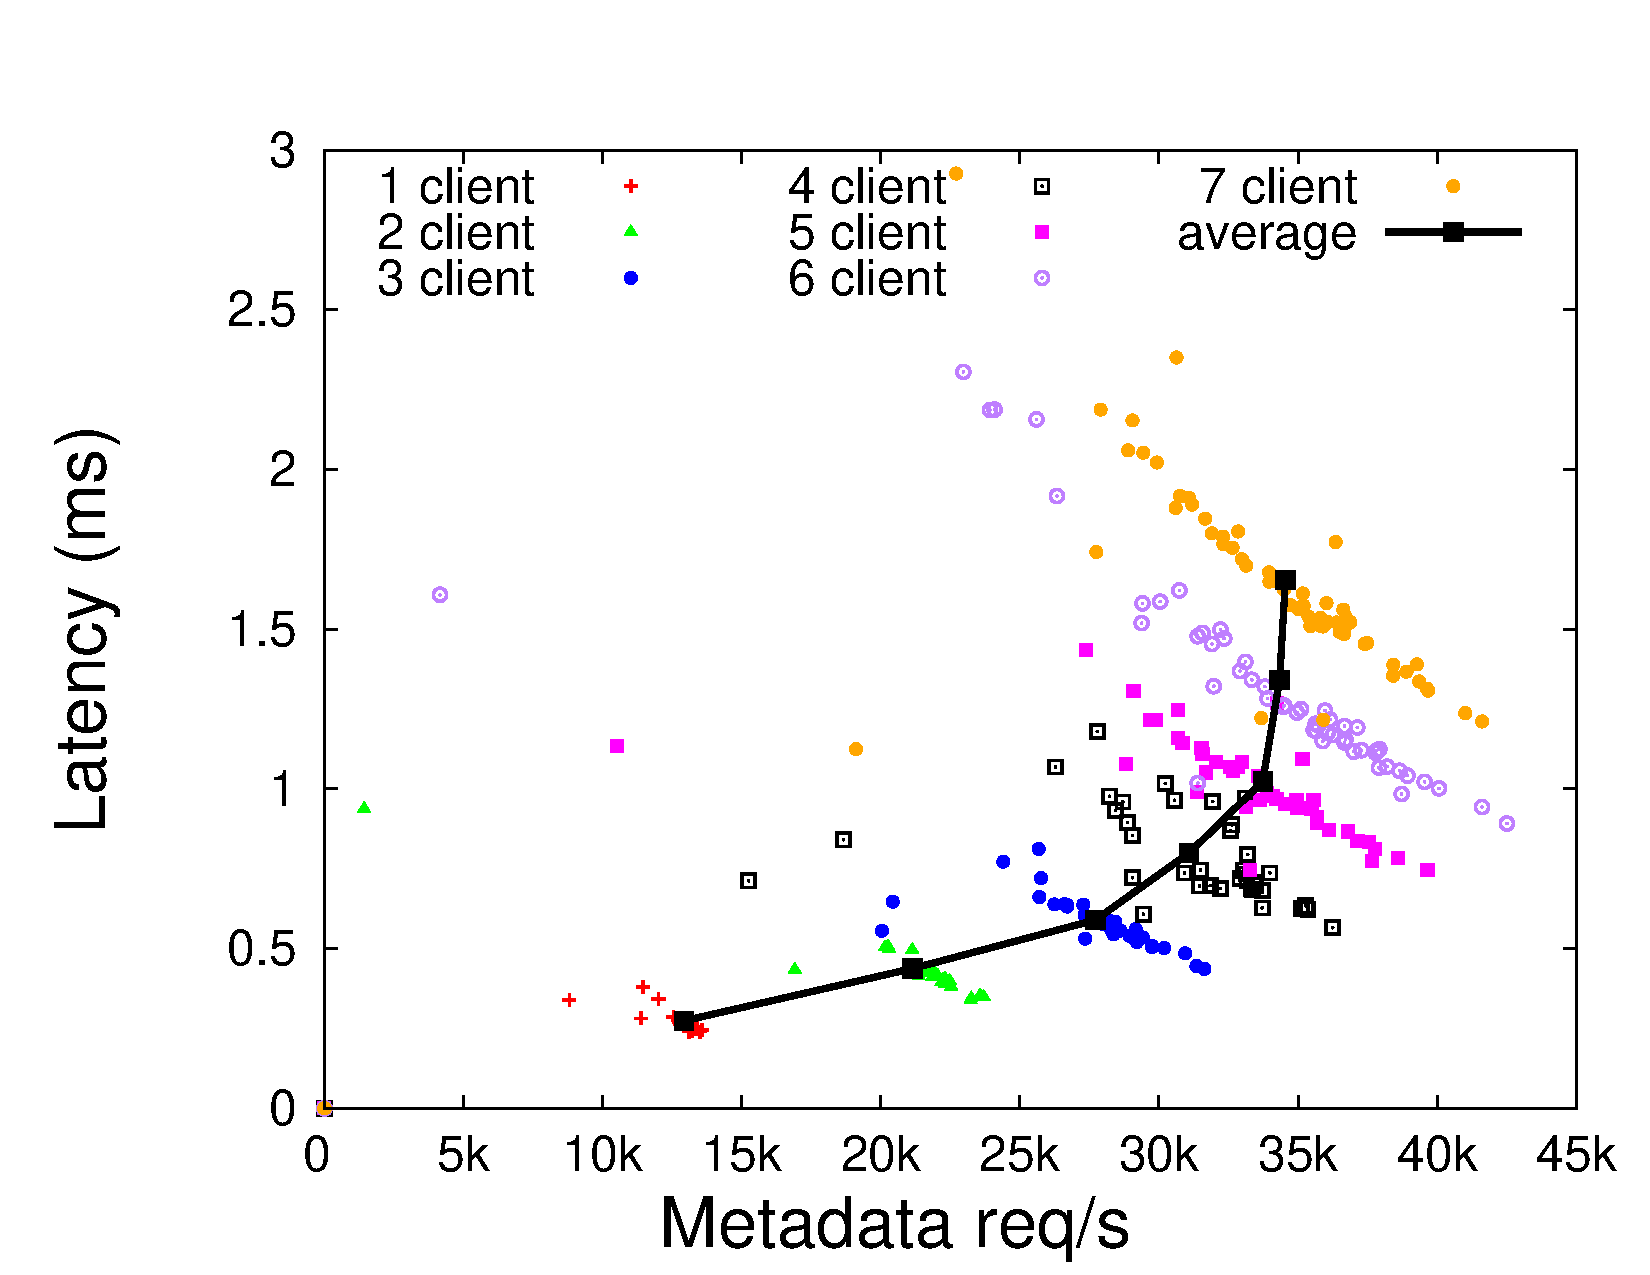
\includegraphics[width=0.45\textwidth]{./chapters/mantle/creates-latency-thruput-clients.pdf}
    \caption{For the create heavy workload, the throughput ({\it x} axis) stops improving and the latency ({\it y} axis) continues to increase with 5, 6, or 7 clients. The standard deviation also increases for latency (up to 3\(\times\)) and throughput (up to 2.3\(\times\)). \label{figure:creates-latency-thruput-clients}} 
\end{figure}

% scalarization 
The CephFS policies, shown in Table~\ref{table:policies}, shape decisions using two techniques: scalarization of logical/physical metrics and hard-coding the logic. Scalarization means collapsing many metrics into a single value, usually with a weighted sum. When partitioning the cluster and the namespace, CephFS calculates metadata and MDS loads by collapsing the logical ({\it e.g.,} inode reads, inode writes, readdirs, etc.) and physical metrics ({\it e.g.,} CPU utilization, memory usage, etc.) into a single value. The exact calculations are in the ``metaload" and ``MDS load'' rows of Table~\ref{table:policies}. 

% Hard code
The other technique CephFS uses in its policies is to compile the decision logic into the system. The balancer uses one approach for deciding when and where to move inodes; it migrates load when it thinks that it has more load than the other MDS nodes (``when" row of Table~\ref{table:policies}) and it tries to migrate enough of its load to make the load even across the MDS cluster (``where" row of Table~\ref{table:policies}). While this approach is scalable, it reduces the efficiency of the cluster if the job could have been completed with less MDS nodes. Figure~\ref{figure:creates-latency-thruput-clients} shows how a single MDS performs as the number of clients is scaled, where each client is creating 100,000 files in separate directories. With an overloaded MDS servicing 5, 6, or 7 clients, throughput stops improving and latency continues to increase. With 1, 2, and 3 clients, the performance variance is small, with a standard deviation for latency between 0.03 and 0.1 ms and for throughput between 103 and 260 requests/second; with 3 or more clients, performance is unpredictable, with a standard deviation for latency between 0.145 and 0.303 ms and for throughput between 406 and 599 requests/second. This indicates that a single MDS can handle up to 4 clients without being overloaded.

% How we can explore accuracy vs. quickness
Each balancer also sets policies for shedding load from its own namespace.  While partitioning the cluster, each balancer assigns each MDS a target load, which is the load the balancer wants to send to that particular MDS. The balancer starts at its root subtrees and continuously sends the largest subtree or dirfrag until reaching this target load (``how-much accuracy" row of Table~\ref{table:policies}). If the target is not reached, the balancer ``drills" down into the hierarchy. This heuristic can lead to poor decisions. For example, in one of our create heavy runs we had 2 MDS nodes, where MDS0 had 8 ``hot" directory fragments with metadata loads: 12.7, 13.3, 13.3, 14.6, 15.7, 13.5, 13.7, 14.6. The balancer on MDS0 tried to ship off half the load by assigning MDS1 a target load of:
\(\frac{\text{total load}}{\text{\# MDSs}} = 55.6\). 
To account for the noise in load measurements, the balancer also scaled the target load by 0.8 (the value of the \texttt{mds\_bal\_need\_min} tunable). As a result, the balancer only shipped off 3 dirfrags, 15.7 + 14.6 + 14.6, instead of half the dirfrags. 

% Why this is set
It is not the case that the balancer cannot decide how much load to send; it is that the balancer is limited to one heuristic (biggest first) to send off dirfrags. We can see why this policy is chosen; it is a fast heuristic to address the bin-packing problem (packing dirfrags onto MDS nodes), which is a combinatorial NP-Hard problem. This approach optimizes the speed of the calculation instead of accuracy and, while it may work for large directories with millions of entries, it struggles with simpler and smaller namespaces because of the noise in the load measurements and calculations.

%%%%%%%%%%%%%%%%%%%%%%%%%%%%%%%%%%%%%%%%%%%%%%%%%%%%%%%%%%%%%%%%%%
\section{Mantle Implementation} 						%%%%%%%%%%
\label{mantle-implementation}							%%%%%%%%%%
%%%%%%%%%%%%%%%%%%%%%%%%%%%%%%%%%%%%%%%%%%%%%%%%%%%%%%%%%%%%%%%%%%
\begin{figure*}
	\centering
	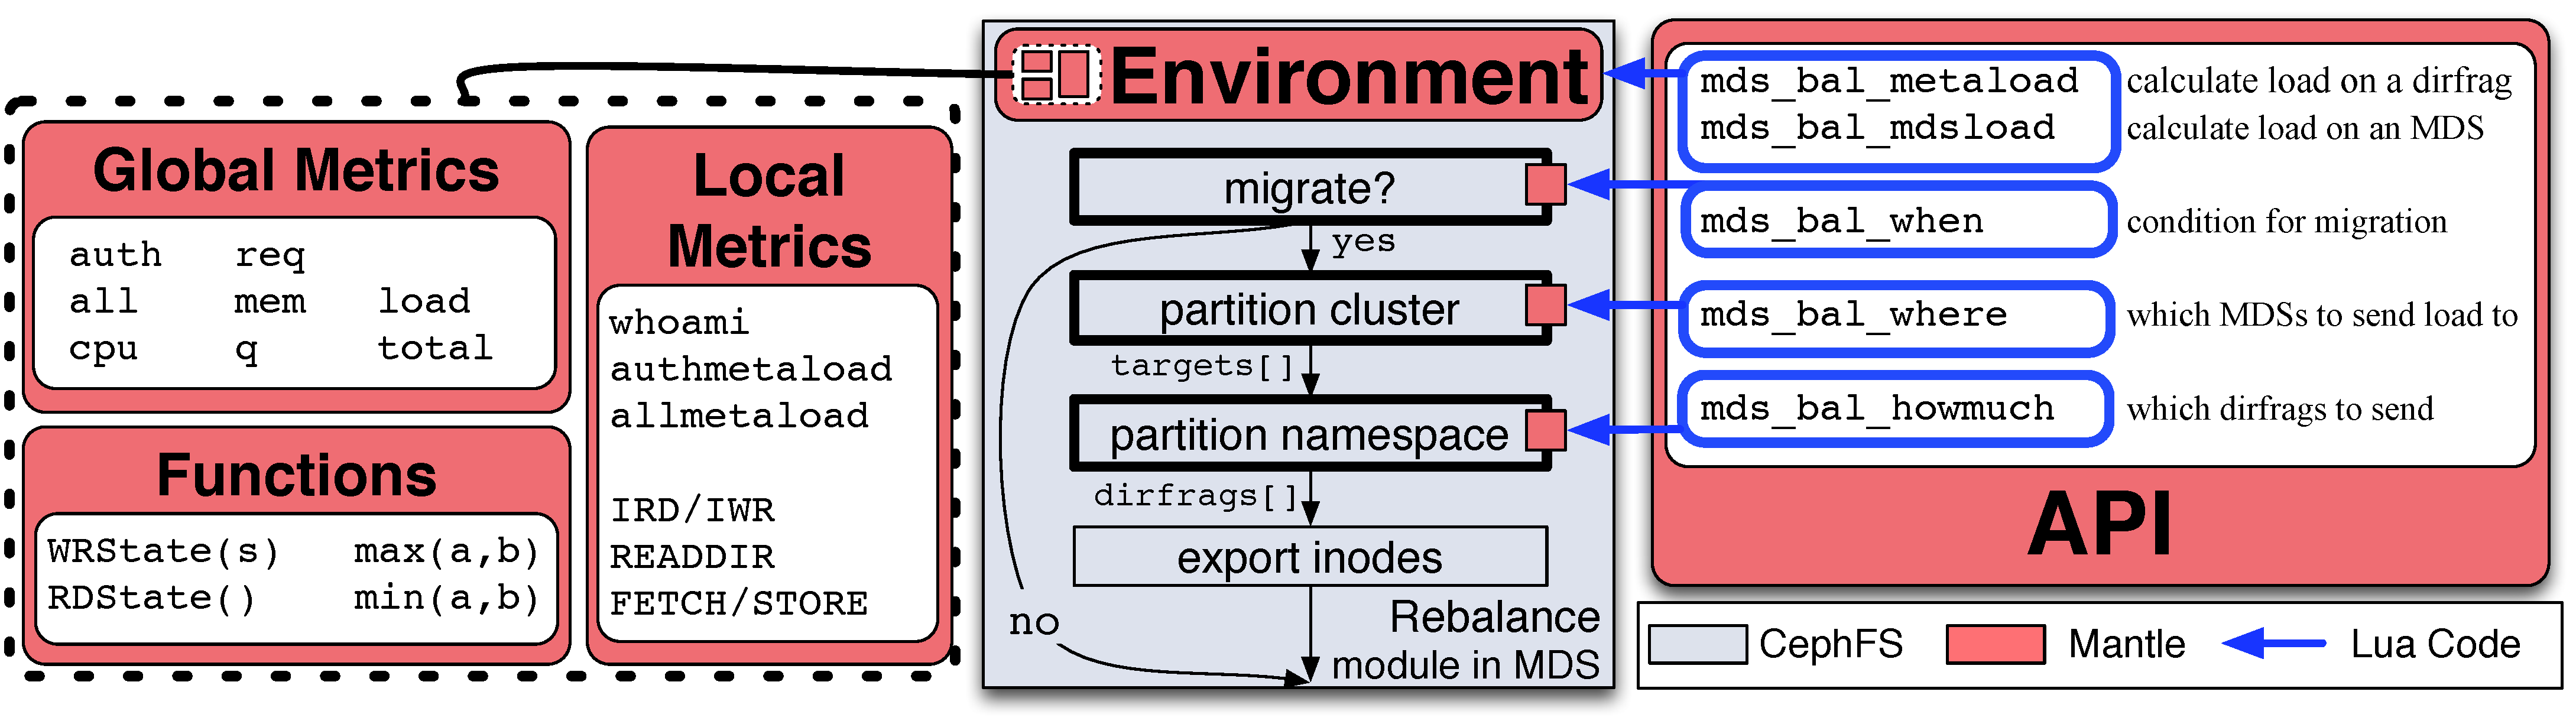
\includegraphics[width=1\textwidth]{./chapters/mantle/balancer-api.pdf} 
	\caption{Designers set policies using the Mantle API. The injectable code uses the metrics/functions in the environment. \label{figure:balancer-api}}  
\end{figure*}

% why we can poke holes
The CephFS policies shape the decision making to be decentralized, aggressive, fast, and slightly forgetful. While these policies work for some workloads, including the workloads used to benchmark CephFS~\cite{weil:sc2004-dyn-metadata}, they do not work for others (as demonstrated in Figure~\ref{figure:creates-thruput}), they underutilize MDS nodes by spreading load to all MDS nodes even if the job could be finished with a subset, they destroy locality by distributing metadata without considering the workload, and they make it harder to coalesce the metadata back to one server after the flash crowd. We emphasize that the problem is that the policies are hardwired into the system, not the policies themselves. 

% Benefits of decoupling
Decoupling the policies from the mechanisms has many advantages: it gives future designers the flexibility to explore the trade-offs of different policies without fear of breaking the system, it keeps the robustness of well-understood implementations intact when exploring new policies, and it allows policies to evolve with new technologies and hardware. For example, McKusick~\cite{mckusick:fast2015-FFS} made the observation that when designing the block allocation mechanism in the Fast File System (FFS), decoupling policy from mechanism greatly enhanced the usability, efficiency, and effectiveness of the system. The low-level allocation mechanism in the FFS has not changed since 1982, but now the developer can try many different policies, even the worst policy imaginable, and the mechanism will never curdle the file system, by doing things like double allocating. 

% What we retained:
Mantle builds on the implementations and data structures in the CephFS balancer, as shown in Figure~\ref{figure:balancer-api}. The mechanisms for dynamic subtree partitioning, including directory fragmentation, moving inodes from one MDS to another, and the exchange of heartbeats, are left unmodified. While this is a standard technique, applying it to a new problem can still be novel, particularly where nobody previously realized they were separable or has tried to separate them.

%%%%%%%%%%%%%%%%%%%%
\subsection{The Mantle Environment}
\label{the-mantle-environment}
%%%%%%%%%%%%%%%%%%%%
\begin{table}[tb]
	\centering
	\begin{tabular}{ >{}p{3.1cm} | >{}p{5.1cm}}
    	\centering Current MDS metrics
		& \centering Description
		\tabularnewline\hline	
		\small\texttt{whoami}
		& current MDS 
		\tabularnewline
		\small\texttt{authmetaload}
		& metadata load on authority subtree
		\tabularnewline	        
		\small\texttt{allmetaload}
		& metadata load on all subtrees
		\tabularnewline	     
		\small\texttt{IRD,IWR}
		& \# inode reads/writes (with a decay)
		\tabularnewline
		\small\texttt{READDIR,FETCH,STORE}
		& \# read directories, fetches, stores
		\tabularnewline	                
        \multicolumn{2}{c}{}
        \tabularnewline
       
		\centering Metrics on MDS {\it i}
		& \centering Description
		\tabularnewline\hline       
		\small\texttt{MDSs[i]["auth"]}	
		& metadata load on authority subtree
		\tabularnewline			
		\small\texttt{MDSs[i]["all"]}	
		& metadata load on all subtrees
		\tabularnewline	        
		\small\texttt{MDSs[i]["cpu"]}
		& \% of total CPU utilization
		\tabularnewline	
		\small\texttt{MDSs[i]["mem"]}	
		& \% of memory utilization
		\tabularnewline	
		\small\texttt{MDSs[i]["q"]}	
		& \# of requests in queue
		\tabularnewline
		\small\texttt{MDSs[i]["req"]}	
		& request rate, in req/sec
		\tabularnewline				
		\small\texttt{MDSs[i]["load"]}	
		& result of \texttt{mds\_bal\_mdsload}
        \tabularnewline
		\small\texttt{total}
		& sum of the load on each MDS        
        \tabularnewline
        \multicolumn{2}{c}{}
        \tabularnewline
        
		\centering Global Functions
		& \centering Description
		\tabularnewline\hline	 
		\small\texttt{WRstate(s)}
		& save state \texttt{s}
        \tabularnewline
        \small\texttt{RDstate()}	
		& read state left by previous decision
        \tabularnewline
        \small\texttt{max(a,b),min(a,b)}
        & get the max, min of two numbers
	\end{tabular}
	\caption{The Mantle environment.\label{table:metrics}}    
\end{table}
Mantle decouples policy from mechanism by letting the designer inject code to control 4 policies: load calculation, ``when" to move load, ``where" to send load, and the accuracy of the decisions. Mantle balancers are written in Lua because Lua is fast (the LuaJIT virtual machine achieves near native performance) and it runs well as modules in other languages~\cite{grawinkel:pdsw2012-lua}. The balancing policies are injected at run time with Ceph's command line tool, {\it e.g.,} \texttt{\small ceph tell mds.0 injectargs mds\_bal\_metaload IWR}. This command means ``tell MDS 0 to calculate load on a dirfrag by the number of inode writes".

% Global variables
Mantle provides a general environment with global variables and functions, shown on the left side of Figure~\ref{figure:balancer-api}, that injectable code can use. Local metrics are the current values for the metadata loads and are usually used to account for the difference between the stale global load and the local load. The library extracts the per-MDS metrics from the MDS heartbeats and puts the global metrics into an MDSs array. The injected code accesses the metric for MDS {\it i} using MDSs[i][``metric"]. The metrics and functions are described in detail in Table~\ref{table:metrics}. The labeled arrows between the phases in Figure~\ref{figure:balancer-api} are the inputs and outputs to the phases; inputs can be used and outputs must be filled by the end of the phase.

% WR/ReadState
The \texttt{WRstate} and \texttt{RDstate} functions help the balancer ``remember'' decisions from the past. For example, in one of the balancers, we wanted to make migration decisions more conservative, so we used \texttt{WRstate} and \texttt{RDstate} to trigger migrations only if the MDS is overloaded for 3 straight iterations. These are implemented using temporary files but future work will store them in RADOS objects to improve scalability.

%%%%%%%%%%%%%%%%%%%%
\subsection{The Mantle API}
\label{the-mantle-api}
%%%%%%%%%%%%%%%%%%%%
% What we did
Figure~\ref{figure:balancer-api} shows where the injected code fits into CephFS: the load calculations and ``when'' code is used in the ``migrate?" decision, the ``where'' decision is used when partitioning the cluster, and the ``howmuch'' decision is used when partitioning the namespace for deciding the accuracy of sending dirfrags. To introduce the API we use the original CephFS balancer as an example. 

\textbf{Metadata/MDS Loads}: these load calculations quantify the work on a subtree/dirfrag and MDS. Mantle runs these calculations and stuffs the results in the \texttt{auth}/\texttt{all} and \texttt{load} variables of Table~\ref{table:metrics}, respectively. To mimic the scalarizations in the original CephFS balancer, one would set \texttt{mds\_} \texttt{bal\_}\texttt{metaload} to:

{\small\begin{verbatim}
IRD + 2*IWR + READDIR + 2*FETCH + 4*STORE
\end{verbatim}}

\noindent and \texttt{mds\_bal\_mdsload} to:

{\small\begin{verbatim}
0.8*MDSs[i]["auth"] + 0.2*MDSs[i]["all"]
+ MDSs[i]["req"] + 10*MDSs[i]["q"]
\end{verbatim}}

The metadata load calculation values inode reads (IRD) less than the writes (IWR), fetches and stores, and the MDS load emphasizes the queue length as a signal that the MDS is overloaded, more than the request rate and metadata loads. 

\textbf{When}: this hook is specified as an ``if'' statement. If the condition evaluates to true, then migration decisions will be made and inodes may be migrated. If the condition is false, then the balancer exits immediately. To implement the original balancer, set \texttt{mds\_bal\_when} to:

{\small\begin{verbatim}
if MDSs[whoami]["load"] > total/#MDSs then
\end{verbatim}}

This forces the MDS to migrate inodes if the load on itself is larger than the average cluster load. This policy is dynamic because it will continually shed load if it senses cluster imbalance, but it also has the potential to thrash load around the cluster if the balancer makes poor decisions. 

\textbf{Where}: the designer specifies where to send load by populating the \texttt{targets} array. The index is the MDS number and the value is set to how much load to send. For example, to send off half the load to the next server, round robin, set \texttt{mds\_bal\_where} to:

{\small\begin{verbatim}
targets[i] = MDSs[whoami + 1]["load"]/2
\end{verbatim}}

The user can also inject large pieces of code. The original CephFS ``where'' balancer can be implemented in 20 lines of Lua code (not shown). 

\textbf{How Much}: recall that the original balancer sheds load by traversing down the namespace and shedding load until reaching the target load for each of the remote MDS nodes. Mantle traverses the namespace in the same way, but exposes the policy for how much to move at each level. Every time Mantle considers a list of dirfrags or subtrees in a directory, it transfers control to an external Lua file with a list of strategies called dirfrag selectors. The dirfrag selectors choose the dirfrags to ship to a remote MDS, given the target load. The ``howmuch" injectable argument accepts a list of dirfrag selectors and the balancer runs all the strategies, selecting the dirfrag selector that gets closest to the target load. We list some of the Mantle example dirfrag selectors below:
\begin{enumerate}\itemsep -2pt
%	\item send biggest dirfrags: \hfill MDS0=66.5, MDS1= 44.7
%	\item send biggest + 1: \hfill MDS0=52.8, MDS1= 58.4	
%	\item send smallest dirfrags: \hfill MDS0=58.4, MDS1= 52.8
%	\item send smallest + 1: \hfill MDS0=44.7, MDS1= 66.5	
%	\item alternate big/small: \hfill MDS0=68.4, MDS1= 42.8	
%	\item alternate big/small + 1: \hfill MDS0=55.1, MDS1= 56.1		
	\item \texttt{big\_first}: biggest dirfrags until reaching target
%	\item[] {\tiny\(15.5+14.6+14.6+13.7\) \hfill MDS0=66.5, MDS1= 44.7}
	\item \texttt{small\_first}: smallest dirfrags until reaching target
%	\item[] {\tiny\(12.7+13.3+13.3+13.5+13.7\)\hfill MDS0=44.7, MDS1= 66.5}
	\item \texttt{big\_small}: alternate sending big and small dirfrags
%	\item[] {\tiny\(15.5+12.7+14.6+13.3\) \hfill MDS0=55.1, MDS1= 56.1}
	\item \texttt{half}: send the first half of the dirfrags
%	\item[] {\tiny\(12.7+13.3+13.3+14.6\) \hfill MDS0=57.3, MDS1= 53.9}
\end{enumerate}
If these dirfrag selectors were running for the problematic dirfrag loads in Section~\S\ref{the-cephfs-policies} (12.7, 13.3, 13.3, 14.6, 15.7, 13.5, 13.7, 14.6),  Mantle would choose the \texttt{big\_small} dirfrag selector because the distance between the target load (55.6) and the load actually shipped is the smallest (0.5). To use the same strategy as the original balancer, set \texttt{mds\_bal\_how\-much} to: \texttt{\{"big\_first"\}}

% Explain that we don't control the actual selection of the subtrees
This hook does not control which subtrees are actually selected during namespace traversal ({\it i.e.} ``which part"). Letting the administrator select specific directories would not scale with the namespace and could be achieved with separate mount points. Mantle uses one approach for traversing the namespace because starting at the root and drilling down into directories ensures the highest spatial and temporal locality, since subtrees are divided and migrated only if their ancestors are too popular to migrate. Policies that influence decisions for dividing, coalescing, or migrating specific subtrees based on other types of locality ({\it e.g.,} request type) are left as future work.

%%%%%%%%%%%%%%%%%%%%%%%%%%%%%%%%%%%%%%%%%%%%%%%%%%%%%%%%%%%%%%%%%%
\section{Evaluation}									%%%%%%%%%%
\label{evaluation}										%%%%%%%%%%
%%%%%%%%%%%%%%%%%%%%%%%%%%%%%%%%%%%%%%%%%%%%%%%%%%%%%%%%%%%%%%%%%%
% Experimental setup
All experiments are run on a 10 node cluster with 18 object storage daemons (OSDs), 1 monitor node (MON), and up to 5 MDS nodes. Each node is running Ubuntu 12.04.4 (kernel version 3.2.0-63) and they have 2 dual core 2GHz processors and 8GB of RAM. There are 3 OSDs per physical server and each OSD has its own disk formatted with XFS for data and an SSD partition for its journal. We use Ceph version 0.91-365-g2da2311. Before each experiment, the cluster is torn down and re-initialized and the kernel caches on all OSDs, MDS nodes, and clients are dropped. 

Performance numbers are specific to CephFS but our contribution is the balancing API/framework that allows users to study different strategies {\it on the same storage system}.  Furthermore, we are not arguing that Mantle is more scalable or better performing than GIGA+, rather, we want to highlight its strategy in comparison to other strategies using Mantle. While it is natural to compare raw performance numbers, we feel (and not just because GIGA+ outperforms Mantle) that we are attacking an orthogonal issue by providing a system for which we can test the strategies of the systems, rather than the systems themselves. 

% Workload discussion
\textbf{Workloads}: we use a small number of workloads to show a comprehensive view of how load is split across MDS nodes. We use file-create workloads because they stress the system, are the focus of other state-of-the-art metadata systems, and they are a common HPC problem (checkpoint/restart). We use compiling code as the other workload because it has different metadata request types/frequencies and because users plan to use CephFS as a shared file system~\cite{website:ceph-cephfs-product-release}. Initial experiments with 1 client compiling with 1 MDS are, admittedly, not interesting, but we use it as a baseline for comparing against setups with more clients. 

% Metrics discussion
\textbf{Metrics}: Mantle pulls out metrics that could be important so that the administrator can freely explore them. The metrics we use are instantaneous CPU utilization and metadata writes, but future balancers will use metrics that better indicate load and that have less variability. In this paper, the high variance in the measurements influences the results of our experiments.

% Balancer design discussion
\textbf{Balancing Heuristics}: we use Mantle to explore techniques from related work: ``Greedy Spill" is from GIGA+, ``Fill \& Spill" is a variation of LARD~\cite{pai:asplos1998}, and the ``Adaptable Balancer" is the original CephFS policy. These heuristics are just starting points and we are not ready to make grandiose statements about which is best. 

%%%%%%%%%%
\subsection{Greedy Spill Balancer}
\label{greedy-spill-balancer}
%%%%%%%%%%
% /user/msevilla/results/sc/spill-evenly
\begin{figure}[tb]
	\centering	
	%\includegraphics[width=0.4\textwidth]{./figures/eval_spill-evenly.pdf}
   	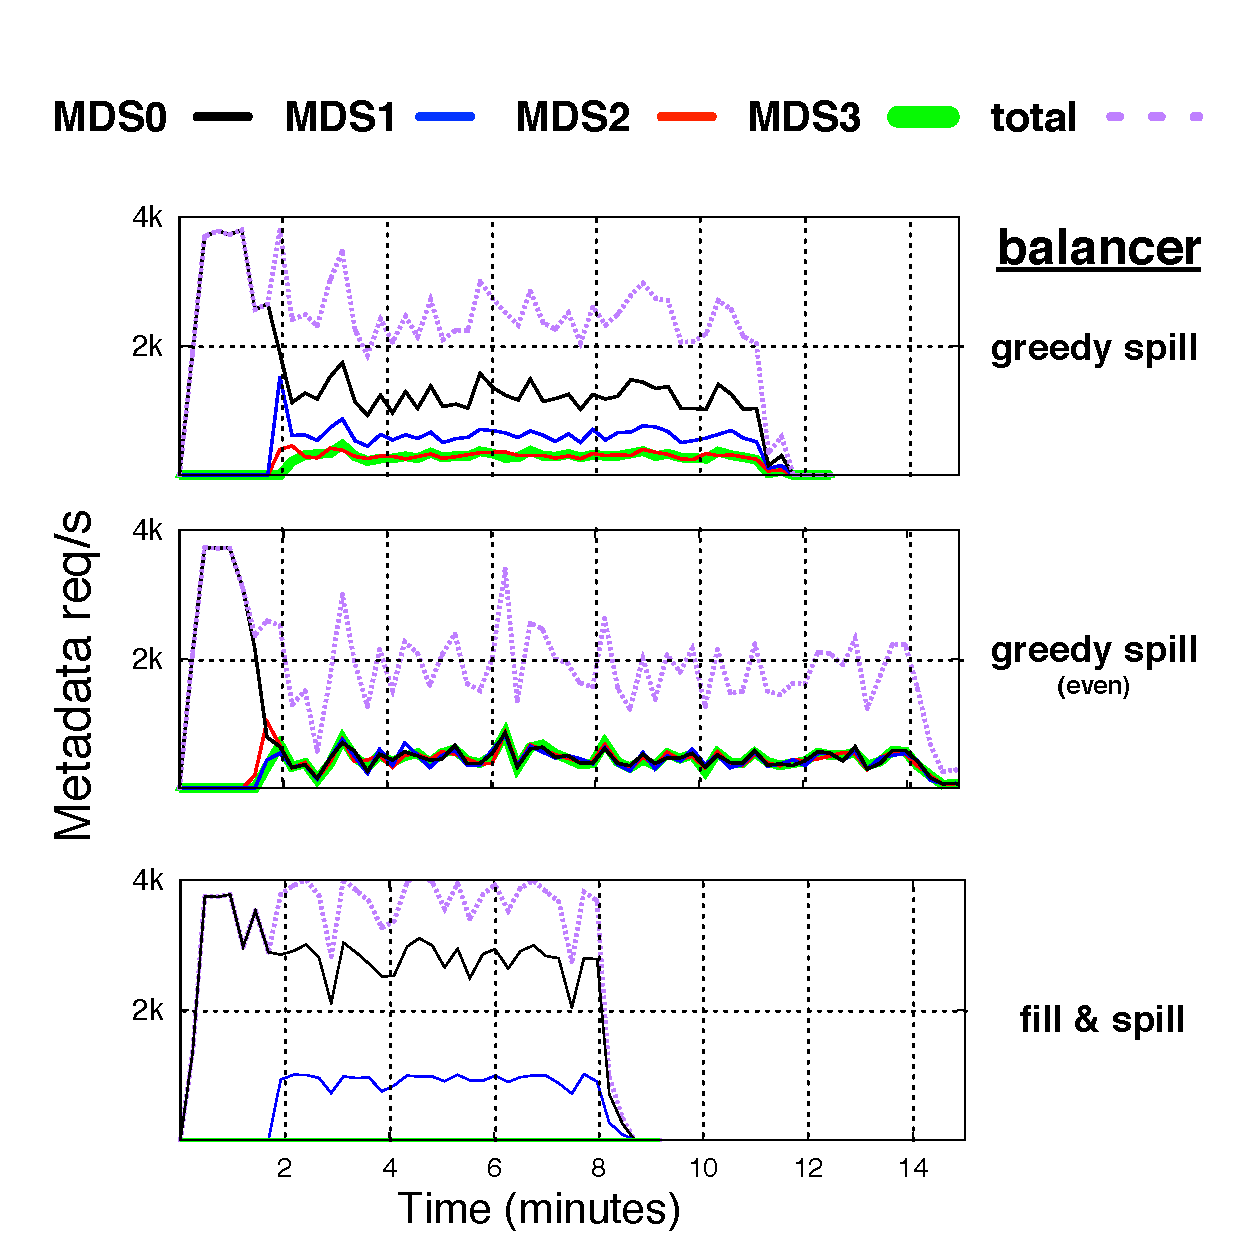
\includegraphics[width=0.4\textwidth]{./chapters/mantle/spill-evenly.pdf}
	\caption{With clients creating files in the same directory, spilling load unevenly with Fill \& Spill has the highest throughput (curves are not stacked), which can have up to 9\% speedup over 1 MDS. Greedy Spill sheds half its metadata immediately while Fill \& Spill sheds part of its metadata when overloaded.\label{figure:eval_spill-evenly}}
\end{figure}
\begin{figure}[tb]
	\centering	
	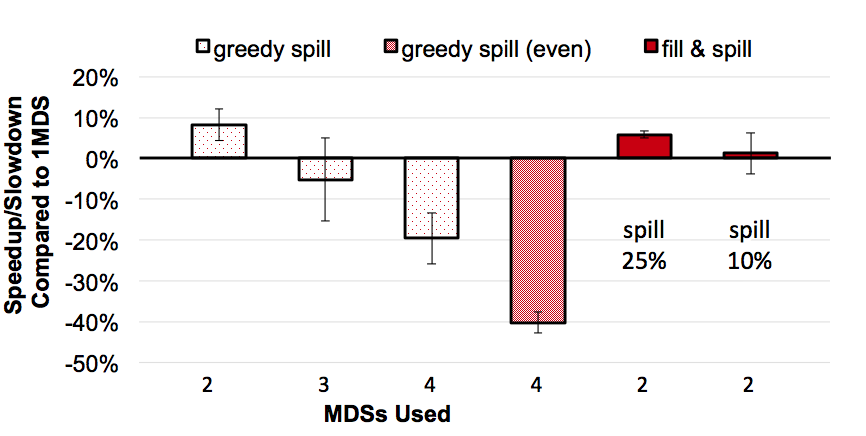
\includegraphics[width=0.4\textwidth]{./chapters/mantle/eval_spill-evenly_bar}
	\caption{The per-client speedup or slowdown shows whether distributing metadata is worthwhile.  Spilling load to 3 or 4 MDS nodes degrades performance but spilling to 2 MDS nodes improves performance.\label{figure:eval_spill-evenly_bar}}
\end{figure}

% overview
This balancer, shown in Listing~\ref{listing:greedy-spill}, aggressively sheds load to all MDS nodes and works well for many clients creating files in the same directory. This balancing strategy mimics the uniform hashing strategy of GIGA+~\cite{patil:fast2011-giga+, ren:sc2014-indexfs}. In these experiments, we use 4 clients each creating 100,000 files in the same directory. When the directory reaches 50,000 directory entries, it is fragmented (the first iteration fragments into \(2^{3}\) = 8 dirfrags) and the balancer migrates half of its dirfrags to an ``underutilized" neighbor. 

\begin{listing}
	\begin{minted}[frame=lines]{lua}
-- Metadata load
metaload = IWR
-- Metadata server load
mdsload = MDSs[i]["all"]
-- When policy
if MDSs[whoami]["load"]>.01 and 
   MDSs[whoami+1]["load"]<.01 then
-- Where policy
targets[whoami+1]=allmetaload/2
-- Howmuch policy
{"half"}
	\end{minted}
    \caption{Greedy Spill Balancer using the Mantle environment (listed in Table~\ref{table:metrics}). Note that all subsequent balancers use the same metadata and MDS loads.\label{listing:greedy-spill}}
\end{listing}

% describe injectable code
The metadata load for the subtrees/dirfrags in the namespace is calculated using just the number of inode writes; we focus on create-intensive workloads, so inode reads are not considered. The MDS load for each MDS is based solely on the metadata load. The balancer migrates load (``when") if two conditions are satisfied: the current MDS has load to migrate and the neighbor MDS does not have any load. If the balancer decides to migrate, it sheds half of the load to its neighbor (``where"). Finally, to ensure that exactly half of the load is sent at each iteration, we employ a custom fragment selector that sends half the dirfrags (``howmuch"). 

% describe results 
The first graph in Figure~\ref{figure:eval_spill-evenly} shows the instantaneous throughput ({\it y} axis) of this balancer over time ({\it x} axis). The MDS nodes spill half their load as soon as they can - this splits load evenly for 2 MDS nodes, but with 4 MDS nodes the load splits unevenly because each MDS spills less load than its predecessor MDS. To get the even balancing shown in the second graph of Figure~\ref{figure:eval_spill-evenly}, the balancer is modified according to Listing~\ref{listing:greedy-spill-evenly} to partition the cluster when selecting the target MDS.
\begin{listing}
	\begin{minted}[frame=lines]{lua}
-- When policy
t=((#MDSs-whoami+1)/2)+whoami
if t>#MDSs then t=whoami end
while t~=whoami and MDSs[t]<.01 do t=t-1 end
if MDSs[whoami]["load"]>.01 and        
   MDSs[t]["load"]<.01 then
-- Where policy
targets[t]=MDSs[whoami]["load"]/2
	\end{minted}
    \caption{Greedy Spill Evenly Balancer.\label{listing:greedy-spill-evenly}}
\end{listing}

% injectable code
This change makes the balancer search for an underloaded MDS in the cluster. It splits the cluster in half and iterates over a subset of the MDS nodes in its search for an underutilized MDS. If it reaches itself or an undefined MDS, then it has nowhere to migrate its load and it does not do any migrations. The ``where" decision uses the target, \texttt{t}, discovered in the ``when" search. With this modification, load is split evenly across all 4 MDS nodes.

% the overall results
The balancer with the most speedup is the 2 MDS configuration, as shown in Figure~\ref{figure:eval_spill-evenly_bar}. This agrees with the assessment of the capacity of a single MDS in Section~\S\ref{setting-policies-for-migration-decisions}; at 4 clients, a single MDS is only slightly overloaded, so splitting load to two MDS nodes only improves the performance by 10\%. Spilling unevenly to 3 and 4 MDS nodes degrades performance by 5\% and 20\% because the cost of synchronizing across multiple MDS nodes penalizes the balancer enough to make migration inefficient. Spilling evenly with 4 MDSs degrades performance up to 40\%  but has the lowest standard deviation because the MDS nodes are underutilized.

% explain the reasons for the poor performance
The difference in performance is dependent on the number of flushes to client sessions. Client sessions ensure coherency and consistency in the file system ({\it e.g.,} permissions, capabilities, etc.) and are flushed when slave MDS nodes rename or migrate directories\footnote{The cause of the latency could be from a scatter-gather process used to exchange statistics with the authoritative MDS. This requires each MDS to halt updates on that directory, send the statistics to the authoritative MDS, and then wait for a response with updates.}: 157 sessions for 1 MDS, 323 session for 2 MDS nodes, 458 sessions for 3 MDS nodes, 788 sessions for 4 MDS nodes spilled unevenly, and 936 sessions for 4 MDS nodes with even metadata distribution. There are more sessions when metadata is distributed because each client contacts MDS nodes round robin for each create. This design decision stems from CephFS's desire to be a general purpose file system, with coherency and consistency for shared resources.\\

\noindent\textbf{Performance}: migration can have such large overhead that the parallelism benefits of distribution are not worthwhile.\\
\noindent\textbf{Stability}: distribution lowers standard deviations because MDS nodes are not as overloaded.

%%%%%%%%%%%%%%%%%%%%%%%%%%%%%%%%%%%%%%%%%%%%%%%%%%%%%%%%%%%%%%%%%%
\subsection{Fill and Spill Balancer}					%%%%%%%%%%
\label{fill-and-spill-balancer}							%%%%%%%%%%
%%%%%%%%%%%%%%%%%%%%%%%%%%%%%%%%%%%%%%%%%%%%%%%%%%%%%%%%%%%%%%%%%%
% overview
This balancer, shown in Listing~\ref{listing:fill-and-spill}, encourages MDS nodes to offload inodes {\it only} when overloaded.  Ideally, the first MDS handles as many clients as possible before shedding load, increasing locality and reducing the number of forwarded requests. Figuring out when an MDS is overloaded is a crucial policy for this balancer. In our implementation, we use the MDS's instantaneous CPU utilization as our load metric, although we envision a more sophisticated metric built from a statistical model for future work. To figure out a good threshold, we look at the CPU utilization from the scaling experiment in Section~\S\ref{setting-policies-for-migration-decisions}. We use the CPU utilization when the MDS has 3 clients, about 48\%, since 5, 6, and 7 clients appear to overload the MDS.  

\begin{listing}
	\begin{minted}[frame=lines]{lua}
-- When policy
wait=RDState(); go = 0;
if MDSs[whoami]["cpu"]>48 then
  if wait>0 then WRState(wait-1)
  else WRState(2); go=1; end
else WRState(2) end
if go==1 then
-- Where policy
targets[whoami+1] = MDSs[whoami]["load"]/4
	\end{minted}
    \caption{Fill and Spill Balancer.\label{listing:fill-and-spill}}
\end{listing}
% injectable code
The injectable code for both the metadata load and MDS load is based solely on the inode reads and writes. The ``when" code forces the balancer to spill when the CPU load is higher than 48\% for more than 3 straight iterations. We added the ``3 straight iterations'' condition to make the balancer more conservative after it had already sent load; in early runs the balancer would send load, then would receive the remote MDS's heartbeat (which is a little stale) and think that the remote MDS is {\it still underloaded}, prompting the balancer to send more load. Finally, the ``where" code tries to spill small load units, just to see if that alleviates load enough to get the CPU utilization back down to 48\%. 

% results
This balancer has a speedup of 6\% over 1 MDS, as shown in Figure~\ref{figure:eval_spill-evenly_bar}, and only uses a subset of the MDS nodes. With 4 available MDS nodes, the balancer only uses 2 of them to complete the job, which minimizes the migrations and the number of sessions. The experiments also show how the amount of spilled load affects performance. Spilling 10\% has a longer runtime, indicating that MDS0 is slightly overloaded when running at 48\% utilization and would be better served if the balancer had shed a little more load. In our experiments, spilling 25\% of the load has the best performance.\\

\noindent\textbf{Performance}: knowing the capacity of an MDS increases performance using only a subset of the MDS nodes.\\
\noindent\textbf{Stability}: the standard deviation of the runtime increases if the balancer compensates for poor migration decisions.

%%%%%%%%%%%%%%%%%%%%%%%%%%%%%%%%%%%%%%%%%%%%%%%%%%%%%%%%%%%%%%%%%%
\subsection{Adaptable Balancer}						%%%%%%%%%%
\label{adaptable-balancer}								%%%%%%%%%%
%%%%%%%%%%%%%%%%%%%%%%%%%%%%%%%%%%%%%%%%%%%%%%%%%%%%%%%%%%%%%%%%%%
\begin{figure}[t]
	\centering	
	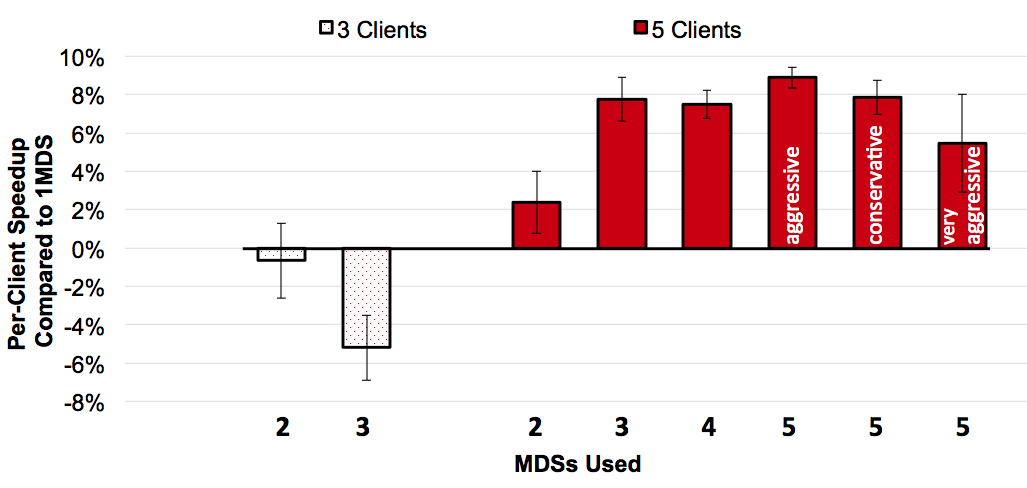
\includegraphics[width=0.5\textwidth]{./chapters/mantle/eval_spill-evenly_compile_bar}\caption{For the compile workload, 3 clients do not overload the MDS nodes so distribution is only a penalty. The speedup for distributing metadata with 5 clients suggests that an MDS with 3 clients is slightly overloaded.  \label{figure:eval_spill-evenly_compile_bar}}
\end{figure}
\begin{figure}[tb]
	\centering	
	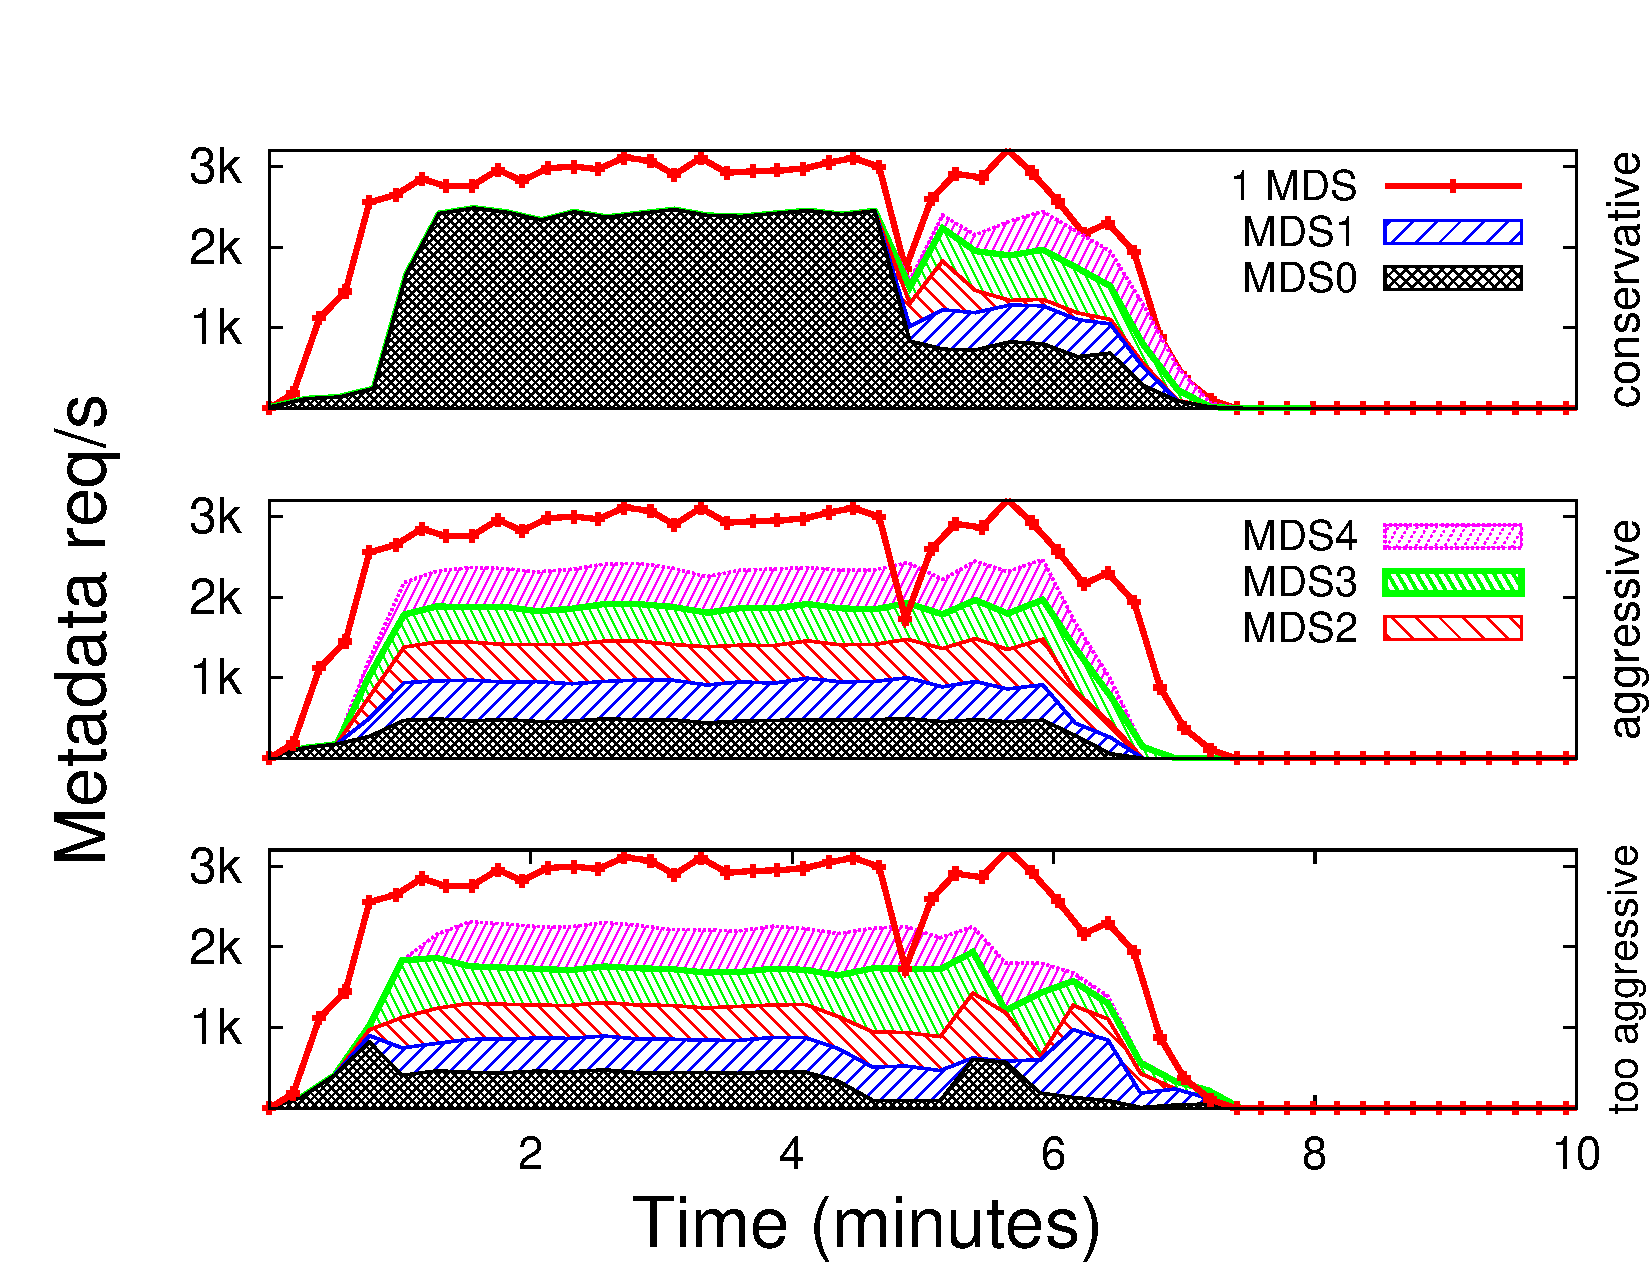
\includegraphics[width=0.45\textwidth]{./chapters/mantle/eval_spill-evenly_compile}\caption{With 5 clients compiling code in separate directories, distributing metadata load early helps the cluster handle a flash crowd at the end of the job. Throughput (stacked curves) drops when using 1 MDS (red curve) because the clients shift to linking, which overloads 1 MDS with \texttt{readdir}s.\label{figure:eval_spill-evenly_compile}}
\end{figure}

This balancer, shown in Listing~\ref{listing:adaptable}, migrates load frequently to try and alleviate hotspots. It works well for dynamic workloads, like compiling code, because it can adapt to the spatial and temporal locality of the requests. The adaptable balancer uses a simplified version of the adaptable load sharing technique of the original balancer.

\begin{listing}
	\begin{minted}[frame=lines]{lua}
-- Metadata load
metaload = IWR + IRD
-- When policy
max=0
for i=1,#MDSs do
  max = max(MDSs[i]["load"], max)
end
myLoad = MDSs[whoami]["load"]
if myLoad>total/2 and myLoad>=max then
-- Balancer where policy
targetLoad=total/#MDSs
for i=1,#MDSs do
  if MDSs[i]["load"]<targetLoad then
    targets[i]=targetLoad-MDSs[i]["load"]
  end
end
-- Howmuch policy
{"half","small","big","big_small"}
	\end{minted}
    \caption{Adaptable Balancer.\label{listing:adaptable}}
\end{listing}

% explain the code
Again, the metadata and MDS loads are set to be the inode writes (not shown). The ``when'' condition only lets the balancer migrate load if the current MDS has more than half the load in the cluster and if it has the most load. This restricts the cluster to only one exporter at a time and only lets that exporter migrate if it has the majority of the load. This makes the migrations more conservative, as the balancer will only react if there is a single MDS that is severely overloaded. The ``where'' code scales the amount of load the current MDS sends according to how much load the remote MDS has. Finally, the balancer tries to be as accurate as possible for all its decisions, so it uses a wide range of dirfrag selectors.

% the results
Figure~\ref{figure:eval_spill-evenly_compile_bar} shows how Mantle can spread load across MDS nodes in different ways. That figure shows the overall performance for 5 clients compiling the Linux source code in separate directories. The balancer immediately moves the large subtrees, in this case the root directory of each client, and then stops migrating because no single MDS has the majority of the load. We conclude that 3 clients do not saturate the system enough to make distribution worthwhile and 5 clients with 3 MDS nodes is just as efficient as 4 or 5 MDS nodes. 

% The performance profile
The performance profile for the 5 MDS setups in Figure~\ref{figure:eval_spill-evenly_compile} shows how the aggressiveness of the balancer affects performance. The bold red curve is the metadata throughput for the compile job with 1 MDS and the stacked throughput curves correspond to the same job with 5 MDS nodes. The top balancer sets a minimum offload number, so it behaves conservatively by keeping all metadata on one MDS until a metadata load spike at 5 minutes forces distribution. The middle balancer is aggressive and distributes metadata load immediately. The flash crowd that triggers the migration in the top graph does not affect the throughput of the aggressive balancer, suggesting that the flash crowd requests metadata that the single MDS setup cannot satisfy fast enough; metadata is subsequently distributed but the flash crowd is already gone. The bottom balancer is far too aggressive and it  tries to achieve perfect balance by constantly moving subtrees/dirfrags. As a result, performance is worse (60\(\times\) as many forwards as the middle balancer), and the standard deviation for the runtime is much higher.\\

\noindent\textbf{Performance}: adapting the system to the workload can improve performance dramatically, but aggressively searching for the perfect balance hurts performance.\\
\noindent\textbf{Stability}: a fragmented namespace destroys locality and influences the standard deviation dramatically.\\
\noindent\textbf{Overhead}: the gap between the 1 MDS curve and the MDS0 curve in the top graph in Figure~\ref{figure:eval_spill-evenly_compile} is the overhead of the balancing logic, which includes the migration decisions, sending heartbeats, and fragmenting directories. The effect is significant, costing almost 500 requests per second, but should be dulled with more MDS nodes if they make decisions independently.

%%%%%%%%%%%%%%%%%%%%%%%%%%%%%%%%%%%%%%%%%%%%%%%%%%%%%%%%%%%%%%%%%%
\subsection{Discussion and Future Work}
\label{discussion-future-work}
%%%%%%%%%%%%%%%%%%%%%%%%%%%%%%%%%%%%%%%%%%%%%%%%%%%%%%%%%%%%%%%%%%
In this paper we only show how certain policies can improve or degrade performance and instead focus on how the API is flexible enough to express many strategies.  While we do not come up with a solution that is better than state-of-the-art systems optimized for file creates ({\it e.g.}, GIGA+), we do present a framework that allows users to study the emergent behavior of different strategies, both in research and in the classroom. In the immediate future, we hope to quantify the effect that policies have on performance by running a suite of workloads over different balancers. Other future endeavors will focus on:

\textbf{Analyzing Scalability}: our MDS cluster is small, but today's production systems use metadata services with a small number of nodes (often less than 5)~\cite{website:ceph-cephfs-product-release}. Our balancers are robust until 20 nodes, at which point there is increased variability in client performance for reasons that we are still investigating. We expect to encounter problems with CephFS's architecture ({\it e.g.}, n-way communication and memory pressure with many files), but we are optimistic that we can try other techniques using Mantle, like GIGA+'s autonomous load splitting, because Mantle MDS nodes independently make decisions. 

%Mantle has already exposed 2 performance deficiencies in CephFS, so it can also help improve metadata protocols and system architectures.	

\textbf{Adding Complex Balancers}: the biggest reason for designing Mantle is to be able to test more complex balancers. Mantle's ability to save state should accommodate balancers that use request cost and statistical modeling, control feedback loops, and machine learning.

\textbf{Analyzing Security and Safety}: in the current prototype, there is little safety - the administrator can inject bad policies ({\it e.g.}, \texttt{while 1}) that brings the whole system down. We wrote a simulator that checks the logic before injecting policies in the running cluster, but this still needs to be integrated into the prototype.


%%%%%%%%%%%%%%%%%%%%%%%%%%%%%%%%%%%%%%%%%%%%%%%%%%%%%%%%%%%%%%%%%%
\section{Related Work}									%%%%%%%%%%
\label{related-work}									%%%%%%%%%%
%%%%%%%%%%%%%%%%%%%%%%%%%%%%%%%%%%%%%%%%%%%%%%%%%%%%%%%%%%%%%%%%%%
% Decouple data/metadata
Mantle decouples policy from mechanism in the metadata service to stabilize decision making. Much of the related work does not focus on the migration policies themselves and instead focuses on mechanisms for moving metadata. 

\textbf{Compute it - Hashing:} this distributes metadata evenly across MDS nodes and clients find the MDS in charge of the metadata by applying a function to a file identifier. PVFSv2~\cite{hildebrand:msst2005-pnfs} and SkyFS~\cite{xing:sc2009-skyfs} hash the filename to locate the authority for metadata. CalvinFS~\cite{thomson:fast2015-calvinfs} hashes the pathname to find a database shard on a server. It handles many small files and fully linearizable random writes using the feature rich Calvin database, which has support for WAN/LAN replication, OLLP for mid-commit commits, and a sophisticated logging subsystem. 

To further enhance scalability, many hashing schemes employ dynamic load balancing. ~\cite{li:msst2006-dynamic} presented dynamic balancing formulas to account for a forgetting factor, access information, and the number of MDS nodes in elastic clusters.~\cite{xing:sc2009-skyfs} used a master-slave architecture to detect low resource usage and migrated metadata using a consistent hashing-based load balancer. GPFS~\cite{schmuck:fast2002-gpfs} elects MDS nodes to manage metadata for different objects. Operations for different objects can operate in parallel and operations to the same object are synchronized. While this approach improves metadata parallelism, delegating management to different servers remains centralized at a token manager. This token manager can be overloaded with requests and large file system sizes - in fact, GPFS actively revokes tokens if the system gets too big. GIGA+~\cite{patil:fast2011-giga+} alleviates hotspots and ``flash crowds" by allowing unsynchronized directory growth for create intensive workloads. Clients contact the parent and traverse down its ``partition history" to find which authority MDS has the data. The follow-up work, IndexFS~\cite{patil:fast2011-giga+}, distributes whole directories to different nodes. To improve lookups and creates, clients cache paths/permissions and metadata logs are stored in a log-structured merge tree for fast insertion and lookup.  Although these techniques improve performance and scalability, especially for create intensive workloads, they do not leverage the locality inherent in file system workloads and they ignore the advantages of keeping the required number of servers to a minimum. 

Many hashing systems achieve locality by adding a metadata cache~\cite{li:msst2006-dynamic, xing:sc2009-skyfs,zhu:pds2008-hba}. For example, Lazy Hybrid~\cite{brandt:mss2003-lh} hashes the filename to locate metadata but maintains extra per-file metadata to manage permissions. Caching popular inodes can help improve locality, but this technique is limited by the size of the caches and only performs well for temporal metadata, instead of spatial metadata locality. Furthermore, cache coherence requires a fair degree of sophistication, limiting its ability to dynamically adapt to the flash crowds.

\textbf{Look it up - Table-based Mapping}: this is a form of hashing, where indices are either managed by a centralized server or the clients. For example, IBRIX~\cite{hp:whitepaper2012-storeall} distributes inode ranges round robin to all servers and HBA~\cite{zhu:pds2008-hba} distributes metadata randomly to each server and uses bloom filters to speedup the table lookups. These techniques also ignore locality.

% website:lustre
\textbf{Traverse it - Subtree Partitioning}: this technique assigns subtrees of the hierarchal namespace to MDS nodes and most systems use a static scheme to partition the namespace at setup, which requires an administrator. Ursa Minor~\cite{sinnamohideen:atc2010-ursa} and Farsite~\cite{doucer:osdi2006-farsite-dir} traverse the namespace to assign related inode ranges, such as inodes in the same subtree, to servers. This benefits performance because the MDS nodes can act independently without synchronizing their actions, making it easy to scale for breadth assuming that the incoming data is evenly partitioned.  Subtree partitioning also gets good locality, making multi-object operations and transactions more efficient. If carefully planned, the metadata distributions can achieve both locality and even load distribution, but their static distribution limits their ability to adapt to hotspots/flash crowds and to maintain balance as data is added.  Some systems, like Panasas~\cite{welch:fast2008-panasas}, allow certain degrees of dynamicity by supporting the addition of new subtrees at runtime, but adapting to the current workload is ignored. 

%Criticism of dynamic subtree partitioning center on implementation details. Related work~\cite{zhu:pds2008-hba, li:msst2006-dynamic} identifies four disadvantages of dynamic subtree partitioning: (1) there is no load measurement scheme/protocol for servers to communicate, (2) adding/removing an MDS requires a directory re-hash, (3) the cost of migrating/coalescing subtrees is unknown, and (4) re-directs around the MDS cluster are costly. These concerns are not related to the technique itself and provide further motivation for exploring dynamic subtree partitioning in more depth. 

\section{Conclusion}
The flexibility of dynamic subtree partitioning introduces significant complexity and many of the challenges that the original balancer tries to address are general, distributed systems problems. In this paper, we present Mantle, a programmable metadata balancer for CephFS that decouples policies from the mechanisms for migration by exposing a general ``balancing" API. We explore the locality vs. distribution space and make important conclusions about the performance and stability implications of migrating load. The key takeaway from using Mantle is that distributing metadata can negatively both performance and stability. With Mantle, we are able to compare the strategies for metadata distribution instead of the underlying systems. With this general framework, broad distributed systems concepts can be explored in depth to gain insights into the true bottlenecks that we face with modern workloads. 
